\documentclass[11pt]{article}
    \usepackage{subcaption}
    \usepackage[breakable]{tcolorbox}
    \usepackage{parskip} % Stop auto-indenting (to mimic markdown behaviour)
    

    % Basic figure setup, for now with no caption control since it's done
    % automatically by Pandoc (which extracts ![](path) syntax from Markdown).
    \usepackage{graphicx}
    % Maintain compatibility with old templates. Remove in nbconvert 6.0
    \let\Oldincludegraphics\includegraphics
    % Ensure that by default, figures have no caption (until we provide a
    % proper Figure object with a Caption API and a way to capture that
    % in the conversion process - todo).
    \usepackage{caption}
    % \DeclareCaptionFormat{nocaption}{}
    % \captionsetup{format=nocaption,aboveskip=0pt,belowskip=0pt}

    \usepackage{float}
    \floatplacement{figure}{H} % forces figures to be placed at the correct location
    \usepackage{xcolor} % Allow colors to be defined
    \usepackage{enumerate} % Needed for markdown enumerations to work
    \usepackage{geometry} % Used to adjust the document margins
    \usepackage{amsmath} % Equations
    \usepackage{amssymb} % Equations
    \usepackage{textcomp} % defines textquotesingle
    % Hack from http://tex.stackexchange.com/a/47451/13684:
    \AtBeginDocument{%
        \def\PYZsq{\textquotesingle}% Upright quotes in Pygmentized code
    }
    \usepackage{upquote} % Upright quotes for verbatim code
    \usepackage{eurosym} % defines \euro

    \usepackage{iftex}
    \ifPDFTeX
        \usepackage[T1]{fontenc}
        \IfFileExists{alphabeta.sty}{
              \usepackage{alphabeta}
          }{
              \usepackage[mathletters]{ucs}
              \usepackage[utf8x]{inputenc}
          }
    \else
        \usepackage{fontspec}
        \usepackage{unicode-math}
    \fi

    \usepackage{fancyvrb} % verbatim replacement that allows latex
    \usepackage{grffile} % extends the file name processing of package graphics
                         % to support a larger range
    \makeatletter % fix for old versions of grffile with XeLaTeX
    \@ifpackagelater{grffile}{2019/11/01}
    {
      % Do nothing on new versions
    }
    {
      \def\Gread@@xetex#1{%
        \IfFileExists{"\Gin@base".bb}%
        {\Gread@eps{\Gin@base.bb}}%
        {\Gread@@xetex@aux#1}%
      }
    }
    \makeatother
    \usepackage[Export]{adjustbox} % Used to constrain images to a maximum size
    \adjustboxset{max size={0.9\linewidth}{0.9\paperheight}}

    % The hyperref package gives us a pdf with properly built
    % internal navigation ('pdf bookmarks' for the table of contents,
    % internal cross-reference links, web links for URLs, etc.)
    \usepackage{hyperref}
    % The default LaTeX title has an obnoxious amount of whitespace. By default,
    % titling removes some of it. It also provides customization options.
    \usepackage{titling}
    \usepackage{longtable} % longtable support required by pandoc >1.10
    \usepackage{booktabs}  % table support for pandoc > 1.12.2
    \usepackage{array}     % table support for pandoc >= 2.11.3
    \usepackage{calc}      % table minipage width calculation for pandoc >= 2.11.1
    \usepackage[inline]{enumitem} % IRkernel/repr support (it uses the enumerate* environment)
    \usepackage[normalem]{ulem} % ulem is needed to support strikethroughs (\sout)
                                % normalem makes italics be italics, not underlines
    \usepackage{mathrsfs}
    

    
    % Colors for the hyperref package
    \definecolor{urlcolor}{rgb}{0,.145,.698}
    \definecolor{linkcolor}{rgb}{.71,0.21,0.01}
    \definecolor{citecolor}{rgb}{.12,.54,.11}

    % ANSI colors
    \definecolor{ansi-black}{HTML}{3E424D}
    \definecolor{ansi-black-intense}{HTML}{282C36}
    \definecolor{ansi-red}{HTML}{E75C58}
    \definecolor{ansi-red-intense}{HTML}{B22B31}
    \definecolor{ansi-green}{HTML}{00A250}
    \definecolor{ansi-green-intense}{HTML}{007427}
    \definecolor{ansi-yellow}{HTML}{DDB62B}
    \definecolor{ansi-yellow-intense}{HTML}{B27D12}
    \definecolor{ansi-blue}{HTML}{208FFB}
    \definecolor{ansi-blue-intense}{HTML}{0065CA}
    \definecolor{ansi-magenta}{HTML}{D160C4}
    \definecolor{ansi-magenta-intense}{HTML}{A03196}
    \definecolor{ansi-cyan}{HTML}{60C6C8}
    \definecolor{ansi-cyan-intense}{HTML}{258F8F}
    \definecolor{ansi-white}{HTML}{C5C1B4}
    \definecolor{ansi-white-intense}{HTML}{A1A6B2}
    \definecolor{ansi-default-inverse-fg}{HTML}{FFFFFF}
    \definecolor{ansi-default-inverse-bg}{HTML}{000000}

    % common color for the border for error outputs.
    \definecolor{outerrorbackground}{HTML}{FFDFDF}

    % commands and environments needed by pandoc snippets
    % extracted from the output of `pandoc -s`
    \providecommand{\tightlist}{%
      \setlength{\itemsep}{0pt}\setlength{\parskip}{0pt}}
    \DefineVerbatimEnvironment{Highlighting}{Verbatim}{commandchars=\\\{\}}
    % Add ',fontsize=\small' for more characters per line
    \newenvironment{Shaded}{}{}
    \newcommand{\KeywordTok}[1]{\textcolor[rgb]{0.00,0.44,0.13}{\textbf{{#1}}}}
    \newcommand{\DataTypeTok}[1]{\textcolor[rgb]{0.56,0.13,0.00}{{#1}}}
    \newcommand{\DecValTok}[1]{\textcolor[rgb]{0.25,0.63,0.44}{{#1}}}
    \newcommand{\BaseNTok}[1]{\textcolor[rgb]{0.25,0.63,0.44}{{#1}}}
    \newcommand{\FloatTok}[1]{\textcolor[rgb]{0.25,0.63,0.44}{{#1}}}
    \newcommand{\CharTok}[1]{\textcolor[rgb]{0.25,0.44,0.63}{{#1}}}
    \newcommand{\StringTok}[1]{\textcolor[rgb]{0.25,0.44,0.63}{{#1}}}
    \newcommand{\CommentTok}[1]{\textcolor[rgb]{0.38,0.63,0.69}{\textit{{#1}}}}
    \newcommand{\OtherTok}[1]{\textcolor[rgb]{0.00,0.44,0.13}{{#1}}}
    \newcommand{\AlertTok}[1]{\textcolor[rgb]{1.00,0.00,0.00}{\textbf{{#1}}}}
    \newcommand{\FunctionTok}[1]{\textcolor[rgb]{0.02,0.16,0.49}{{#1}}}
    \newcommand{\RegionMarkerTok}[1]{{#1}}
    \newcommand{\ErrorTok}[1]{\textcolor[rgb]{1.00,0.00,0.00}{\textbf{{#1}}}}
    \newcommand{\NormalTok}[1]{{#1}}

    % Additional commands for more recent versions of Pandoc
    \newcommand{\ConstantTok}[1]{\textcolor[rgb]{0.53,0.00,0.00}{{#1}}}
    \newcommand{\SpecialCharTok}[1]{\textcolor[rgb]{0.25,0.44,0.63}{{#1}}}
    \newcommand{\VerbatimStringTok}[1]{\textcolor[rgb]{0.25,0.44,0.63}{{#1}}}
    \newcommand{\SpecialStringTok}[1]{\textcolor[rgb]{0.73,0.40,0.53}{{#1}}}
    \newcommand{\ImportTok}[1]{{#1}}
    \newcommand{\DocumentationTok}[1]{\textcolor[rgb]{0.73,0.13,0.13}{\textit{{#1}}}}
    \newcommand{\AnnotationTok}[1]{\textcolor[rgb]{0.38,0.63,0.69}{\textbf{\textit{{#1}}}}}
    \newcommand{\CommentVarTok}[1]{\textcolor[rgb]{0.38,0.63,0.69}{\textbf{\textit{{#1}}}}}
    \newcommand{\VariableTok}[1]{\textcolor[rgb]{0.10,0.09,0.49}{{#1}}}
    \newcommand{\ControlFlowTok}[1]{\textcolor[rgb]{0.00,0.44,0.13}{\textbf{{#1}}}}
    \newcommand{\OperatorTok}[1]{\textcolor[rgb]{0.40,0.40,0.40}{{#1}}}
    \newcommand{\BuiltInTok}[1]{{#1}}
    \newcommand{\ExtensionTok}[1]{{#1}}
    \newcommand{\PreprocessorTok}[1]{\textcolor[rgb]{0.74,0.48,0.00}{{#1}}}
    \newcommand{\AttributeTok}[1]{\textcolor[rgb]{0.49,0.56,0.16}{{#1}}}
    \newcommand{\InformationTok}[1]{\textcolor[rgb]{0.38,0.63,0.69}{\textbf{\textit{{#1}}}}}
    \newcommand{\WarningTok}[1]{\textcolor[rgb]{0.38,0.63,0.69}{\textbf{\textit{{#1}}}}}


    % Define a nice break command that doesn't care if a line doesn't already
    % exist.
    \def\br{\hspace*{\fill} \\* }
    % Math Jax compatibility definitions
    \def\gt{>}
    \def\lt{<}
    \let\Oldtex\TeX
    \let\Oldlatex\LaTeX
    \renewcommand{\TeX}{\textrm{\Oldtex}}
    \renewcommand{\LaTeX}{\textrm{\Oldlatex}}
    % Document parameters
    % Document title
    \title{
    Microarray Gene Expression Analysis\\
    \large Acute myeloid leukemia (AML)
    }
    \author{Saman Dehestani \thanks{401208226} \and Sajede Fadaei \thanks{400211513} \and Aminreza Sefid \thanks{401208204}}

    
    
    
% Pygments definitions
\makeatletter
\def\PY@reset{\let\PY@it=\relax \let\PY@bf=\relax%
    \let\PY@ul=\relax \let\PY@tc=\relax%
    \let\PY@bc=\relax \let\PY@ff=\relax}
\def\PY@tok#1{\csname PY@tok@#1\endcsname}
\def\PY@toks#1+{\ifx\relax#1\empty\else%
    \PY@tok{#1}\expandafter\PY@toks\fi}
\def\PY@do#1{\PY@bc{\PY@tc{\PY@ul{%
    \PY@it{\PY@bf{\PY@ff{#1}}}}}}}
\def\PY#1#2{\PY@reset\PY@toks#1+\relax+\PY@do{#2}}

\@namedef{PY@tok@w}{\def\PY@tc##1{\textcolor[rgb]{0.73,0.73,0.73}{##1}}}
\@namedef{PY@tok@c}{\let\PY@it=\textit\def\PY@tc##1{\textcolor[rgb]{0.24,0.48,0.48}{##1}}}
\@namedef{PY@tok@cp}{\def\PY@tc##1{\textcolor[rgb]{0.61,0.40,0.00}{##1}}}
\@namedef{PY@tok@k}{\let\PY@bf=\textbf\def\PY@tc##1{\textcolor[rgb]{0.00,0.50,0.00}{##1}}}
\@namedef{PY@tok@kp}{\def\PY@tc##1{\textcolor[rgb]{0.00,0.50,0.00}{##1}}}
\@namedef{PY@tok@kt}{\def\PY@tc##1{\textcolor[rgb]{0.69,0.00,0.25}{##1}}}
\@namedef{PY@tok@o}{\def\PY@tc##1{\textcolor[rgb]{0.40,0.40,0.40}{##1}}}
\@namedef{PY@tok@ow}{\let\PY@bf=\textbf\def\PY@tc##1{\textcolor[rgb]{0.67,0.13,1.00}{##1}}}
\@namedef{PY@tok@nb}{\def\PY@tc##1{\textcolor[rgb]{0.00,0.50,0.00}{##1}}}
\@namedef{PY@tok@nf}{\def\PY@tc##1{\textcolor[rgb]{0.00,0.00,1.00}{##1}}}
\@namedef{PY@tok@nc}{\let\PY@bf=\textbf\def\PY@tc##1{\textcolor[rgb]{0.00,0.00,1.00}{##1}}}
\@namedef{PY@tok@nn}{\let\PY@bf=\textbf\def\PY@tc##1{\textcolor[rgb]{0.00,0.00,1.00}{##1}}}
\@namedef{PY@tok@ne}{\let\PY@bf=\textbf\def\PY@tc##1{\textcolor[rgb]{0.80,0.25,0.22}{##1}}}
\@namedef{PY@tok@nv}{\def\PY@tc##1{\textcolor[rgb]{0.10,0.09,0.49}{##1}}}
\@namedef{PY@tok@no}{\def\PY@tc##1{\textcolor[rgb]{0.53,0.00,0.00}{##1}}}
\@namedef{PY@tok@nl}{\def\PY@tc##1{\textcolor[rgb]{0.46,0.46,0.00}{##1}}}
\@namedef{PY@tok@ni}{\let\PY@bf=\textbf\def\PY@tc##1{\textcolor[rgb]{0.44,0.44,0.44}{##1}}}
\@namedef{PY@tok@na}{\def\PY@tc##1{\textcolor[rgb]{0.41,0.47,0.13}{##1}}}
\@namedef{PY@tok@nt}{\let\PY@bf=\textbf\def\PY@tc##1{\textcolor[rgb]{0.00,0.50,0.00}{##1}}}
\@namedef{PY@tok@nd}{\def\PY@tc##1{\textcolor[rgb]{0.67,0.13,1.00}{##1}}}
\@namedef{PY@tok@s}{\def\PY@tc##1{\textcolor[rgb]{0.73,0.13,0.13}{##1}}}
\@namedef{PY@tok@sd}{\let\PY@it=\textit\def\PY@tc##1{\textcolor[rgb]{0.73,0.13,0.13}{##1}}}
\@namedef{PY@tok@si}{\let\PY@bf=\textbf\def\PY@tc##1{\textcolor[rgb]{0.64,0.35,0.47}{##1}}}
\@namedef{PY@tok@se}{\let\PY@bf=\textbf\def\PY@tc##1{\textcolor[rgb]{0.67,0.36,0.12}{##1}}}
\@namedef{PY@tok@sr}{\def\PY@tc##1{\textcolor[rgb]{0.64,0.35,0.47}{##1}}}
\@namedef{PY@tok@ss}{\def\PY@tc##1{\textcolor[rgb]{0.10,0.09,0.49}{##1}}}
\@namedef{PY@tok@sx}{\def\PY@tc##1{\textcolor[rgb]{0.00,0.50,0.00}{##1}}}
\@namedef{PY@tok@m}{\def\PY@tc##1{\textcolor[rgb]{0.40,0.40,0.40}{##1}}}
\@namedef{PY@tok@gh}{\let\PY@bf=\textbf\def\PY@tc##1{\textcolor[rgb]{0.00,0.00,0.50}{##1}}}
\@namedef{PY@tok@gu}{\let\PY@bf=\textbf\def\PY@tc##1{\textcolor[rgb]{0.50,0.00,0.50}{##1}}}
\@namedef{PY@tok@gd}{\def\PY@tc##1{\textcolor[rgb]{0.63,0.00,0.00}{##1}}}
\@namedef{PY@tok@gi}{\def\PY@tc##1{\textcolor[rgb]{0.00,0.52,0.00}{##1}}}
\@namedef{PY@tok@gr}{\def\PY@tc##1{\textcolor[rgb]{0.89,0.00,0.00}{##1}}}
\@namedef{PY@tok@ge}{\let\PY@it=\textit}
\@namedef{PY@tok@gs}{\let\PY@bf=\textbf}
\@namedef{PY@tok@gp}{\let\PY@bf=\textbf\def\PY@tc##1{\textcolor[rgb]{0.00,0.00,0.50}{##1}}}
\@namedef{PY@tok@go}{\def\PY@tc##1{\textcolor[rgb]{0.44,0.44,0.44}{##1}}}
\@namedef{PY@tok@gt}{\def\PY@tc##1{\textcolor[rgb]{0.00,0.27,0.87}{##1}}}
\@namedef{PY@tok@err}{\def\PY@bc##1{{\setlength{\fboxsep}{\string -\fboxrule}\fcolorbox[rgb]{1.00,0.00,0.00}{1,1,1}{\strut ##1}}}}
\@namedef{PY@tok@kc}{\let\PY@bf=\textbf\def\PY@tc##1{\textcolor[rgb]{0.00,0.50,0.00}{##1}}}
\@namedef{PY@tok@kd}{\let\PY@bf=\textbf\def\PY@tc##1{\textcolor[rgb]{0.00,0.50,0.00}{##1}}}
\@namedef{PY@tok@kn}{\let\PY@bf=\textbf\def\PY@tc##1{\textcolor[rgb]{0.00,0.50,0.00}{##1}}}
\@namedef{PY@tok@kr}{\let\PY@bf=\textbf\def\PY@tc##1{\textcolor[rgb]{0.00,0.50,0.00}{##1}}}
\@namedef{PY@tok@bp}{\def\PY@tc##1{\textcolor[rgb]{0.00,0.50,0.00}{##1}}}
\@namedef{PY@tok@fm}{\def\PY@tc##1{\textcolor[rgb]{0.00,0.00,1.00}{##1}}}
\@namedef{PY@tok@vc}{\def\PY@tc##1{\textcolor[rgb]{0.10,0.09,0.49}{##1}}}
\@namedef{PY@tok@vg}{\def\PY@tc##1{\textcolor[rgb]{0.10,0.09,0.49}{##1}}}
\@namedef{PY@tok@vi}{\def\PY@tc##1{\textcolor[rgb]{0.10,0.09,0.49}{##1}}}
\@namedef{PY@tok@vm}{\def\PY@tc##1{\textcolor[rgb]{0.10,0.09,0.49}{##1}}}
\@namedef{PY@tok@sa}{\def\PY@tc##1{\textcolor[rgb]{0.73,0.13,0.13}{##1}}}
\@namedef{PY@tok@sb}{\def\PY@tc##1{\textcolor[rgb]{0.73,0.13,0.13}{##1}}}
\@namedef{PY@tok@sc}{\def\PY@tc##1{\textcolor[rgb]{0.73,0.13,0.13}{##1}}}
\@namedef{PY@tok@dl}{\def\PY@tc##1{\textcolor[rgb]{0.73,0.13,0.13}{##1}}}
\@namedef{PY@tok@s2}{\def\PY@tc##1{\textcolor[rgb]{0.73,0.13,0.13}{##1}}}
\@namedef{PY@tok@sh}{\def\PY@tc##1{\textcolor[rgb]{0.73,0.13,0.13}{##1}}}
\@namedef{PY@tok@s1}{\def\PY@tc##1{\textcolor[rgb]{0.73,0.13,0.13}{##1}}}
\@namedef{PY@tok@mb}{\def\PY@tc##1{\textcolor[rgb]{0.40,0.40,0.40}{##1}}}
\@namedef{PY@tok@mf}{\def\PY@tc##1{\textcolor[rgb]{0.40,0.40,0.40}{##1}}}
\@namedef{PY@tok@mh}{\def\PY@tc##1{\textcolor[rgb]{0.40,0.40,0.40}{##1}}}
\@namedef{PY@tok@mi}{\def\PY@tc##1{\textcolor[rgb]{0.40,0.40,0.40}{##1}}}
\@namedef{PY@tok@il}{\def\PY@tc##1{\textcolor[rgb]{0.40,0.40,0.40}{##1}}}
\@namedef{PY@tok@mo}{\def\PY@tc##1{\textcolor[rgb]{0.40,0.40,0.40}{##1}}}
\@namedef{PY@tok@ch}{\let\PY@it=\textit\def\PY@tc##1{\textcolor[rgb]{0.24,0.48,0.48}{##1}}}
\@namedef{PY@tok@cm}{\let\PY@it=\textit\def\PY@tc##1{\textcolor[rgb]{0.24,0.48,0.48}{##1}}}
\@namedef{PY@tok@cpf}{\let\PY@it=\textit\def\PY@tc##1{\textcolor[rgb]{0.24,0.48,0.48}{##1}}}
\@namedef{PY@tok@c1}{\let\PY@it=\textit\def\PY@tc##1{\textcolor[rgb]{0.24,0.48,0.48}{##1}}}
\@namedef{PY@tok@cs}{\let\PY@it=\textit\def\PY@tc##1{\textcolor[rgb]{0.24,0.48,0.48}{##1}}}

\def\PYZbs{\char`\\}
\def\PYZus{\char`\_}
\def\PYZob{\char`\{}
\def\PYZcb{\char`\}}
\def\PYZca{\char`\^}
\def\PYZam{\char`\&}
\def\PYZlt{\char`\<}
\def\PYZgt{\char`\>}
\def\PYZsh{\char`\#}
\def\PYZpc{\char`\%}
\def\PYZdl{\char`\$}
\def\PYZhy{\char`\-}
\def\PYZsq{\char`\'}
\def\PYZdq{\char`\"}
\def\PYZti{\char`\~}
% for compatibility with earlier versions
\def\PYZat{@}
\def\PYZlb{[}
\def\PYZrb{]}
\makeatother


    % For linebreaks inside Verbatim environment from package fancyvrb.
    \makeatletter
        \newbox\Wrappedcontinuationbox
        \newbox\Wrappedvisiblespacebox
        \newcommand*\Wrappedvisiblespace {\textcolor{red}{\textvisiblespace}}
        \newcommand*\Wrappedcontinuationsymbol {\textcolor{red}{\llap{\tiny$\m@th\hookrightarrow$}}}
        \newcommand*\Wrappedcontinuationindent {3ex }
        \newcommand*\Wrappedafterbreak {\kern\Wrappedcontinuationindent\copy\Wrappedcontinuationbox}
        % Take advantage of the already applied Pygments mark-up to insert
        % potential linebreaks for TeX processing.
        %        {, <, #, %, $, ' and ": go to next line.
        %        _, }, ^, &, >, - and ~: stay at end of broken line.
        % Use of \textquotesingle for straight quote.
        \newcommand*\Wrappedbreaksatspecials {%
            \def\PYGZus{\discretionary{\char`\_}{\Wrappedafterbreak}{\char`\_}}%
            \def\PYGZob{\discretionary{}{\Wrappedafterbreak\char`\{}{\char`\{}}%
            \def\PYGZcb{\discretionary{\char`\}}{\Wrappedafterbreak}{\char`\}}}%
            \def\PYGZca{\discretionary{\char`\^}{\Wrappedafterbreak}{\char`\^}}%
            \def\PYGZam{\discretionary{\char`\&}{\Wrappedafterbreak}{\char`\&}}%
            \def\PYGZlt{\discretionary{}{\Wrappedafterbreak\char`\<}{\char`\<}}%
            \def\PYGZgt{\discretionary{\char`\>}{\Wrappedafterbreak}{\char`\>}}%
            \def\PYGZsh{\discretionary{}{\Wrappedafterbreak\char`\#}{\char`\#}}%
            \def\PYGZpc{\discretionary{}{\Wrappedafterbreak\char`\%}{\char`\%}}%
            \def\PYGZdl{\discretionary{}{\Wrappedafterbreak\char`\$}{\char`\$}}%
            \def\PYGZhy{\discretionary{\char`\-}{\Wrappedafterbreak}{\char`\-}}%
            \def\PYGZsq{\discretionary{}{\Wrappedafterbreak\textquotesingle}{\textquotesingle}}%
            \def\PYGZdq{\discretionary{}{\Wrappedafterbreak\char`\"}{\char`\"}}%
            \def\PYGZti{\discretionary{\char`\~}{\Wrappedafterbreak}{\char`\~}}%
        }
        % Some characters . , ; ? ! / are not pygmentized.
        % This macro makes them "active" and they will insert potential linebreaks
        \newcommand*\Wrappedbreaksatpunct {%
            \lccode`\~`\.\lowercase{\def~}{\discretionary{\hbox{\char`\.}}{\Wrappedafterbreak}{\hbox{\char`\.}}}%
            \lccode`\~`\,\lowercase{\def~}{\discretionary{\hbox{\char`\,}}{\Wrappedafterbreak}{\hbox{\char`\,}}}%
            \lccode`\~`\;\lowercase{\def~}{\discretionary{\hbox{\char`\;}}{\Wrappedafterbreak}{\hbox{\char`\;}}}%
            \lccode`\~`\:\lowercase{\def~}{\discretionary{\hbox{\char`\:}}{\Wrappedafterbreak}{\hbox{\char`\:}}}%
            \lccode`\~`\?\lowercase{\def~}{\discretionary{\hbox{\char`\?}}{\Wrappedafterbreak}{\hbox{\char`\?}}}%
            \lccode`\~`\!\lowercase{\def~}{\discretionary{\hbox{\char`\!}}{\Wrappedafterbreak}{\hbox{\char`\!}}}%
            \lccode`\~`\/\lowercase{\def~}{\discretionary{\hbox{\char`\/}}{\Wrappedafterbreak}{\hbox{\char`\/}}}%
            \catcode`\.\active
            \catcode`\,\active
            \catcode`\;\active
            \catcode`\:\active
            \catcode`\?\active
            \catcode`\!\active
            \catcode`\/\active
            \lccode`\~`\~
        }
    \makeatother

    \let\OriginalVerbatim=\Verbatim
    \makeatletter
    \renewcommand{\Verbatim}[1][1]{%
        %\parskip\z@skip
        \sbox\Wrappedcontinuationbox {\Wrappedcontinuationsymbol}%
        \sbox\Wrappedvisiblespacebox {\FV@SetupFont\Wrappedvisiblespace}%
        \def\FancyVerbFormatLine ##1{\hsize\linewidth
            \vtop{\raggedright\hyphenpenalty\z@\exhyphenpenalty\z@
                \doublehyphendemerits\z@\finalhyphendemerits\z@
                \strut ##1\strut}%
        }%
        % If the linebreak is at a space, the latter will be displayed as visible
        % space at end of first line, and a continuation symbol starts next line.
        % Stretch/shrink are however usually zero for typewriter font.
        \def\FV@Space {%
            \nobreak\hskip\z@ plus\fontdimen3\font minus\fontdimen4\font
            \discretionary{\copy\Wrappedvisiblespacebox}{\Wrappedafterbreak}
            {\kern\fontdimen2\font}%
        }%

        % Allow breaks at special characters using \PYG... macros.
        \Wrappedbreaksatspecials
        % Breaks at punctuation characters . , ; ? ! and / need catcode=\active
        \OriginalVerbatim[#1,codes*=\Wrappedbreaksatpunct]%
    }
    \makeatother

    % Exact colors from NB
    \definecolor{incolor}{HTML}{303F9F}
    \definecolor{outcolor}{HTML}{D84315}
    \definecolor{cellborder}{HTML}{CFCFCF}
    \definecolor{cellbackground}{HTML}{F7F7F7}

    % prompt
    \makeatletter
    \newcommand{\boxspacing}{\kern\kvtcb@left@rule\kern\kvtcb@boxsep}
    \makeatother
    \newcommand{\prompt}[4]{
        {\ttfamily\llap{{\color{#2}[#3]:\hspace{3pt}#4}}\vspace{-\baselineskip}}
    }
    

    
    % Prevent overflowing lines due to hard-to-break entities
    \sloppy
    % Setup hyperref package
    \hypersetup{
      breaklinks=true,  % so long urls are correctly broken across lines
      colorlinks=true,
      urlcolor=urlcolor,
      linkcolor=linkcolor,
      citecolor=citecolor,
      }
    % Slightly bigger margins than the latex defaults
    
    \geometry{verbose,tmargin=1in,bmargin=1in,lmargin=1in,rmargin=1in}
    
    

\begin{document}
    
    \maketitle
    
    

    
    \hypertarget{microarray}{%
\section{Microarray}\label{microarray}}

A microarray is a laboratory tool used to detect the expression of genes
from a sample at the same time.

Microarrays have thousands of tiny spots in defined positions, with each
spot containing a known DNA sequence or gene. The DNA molecules attached
to each slide act as probes to detect gene expression.

To perform a microarray, mRNA molecules are typically collected from two
different groups. For example, one group is considered as reference,
which includes healthy samples and another group is experimental samples
collected from a disease individual such as cancer.

The two mRNA samples are then converted into complementary DNA (cDNA)
and each sample is labeled with a fluorescent probe of a different
color. For instance, the experimental cDNA may be labeled with a red
fluorescent dye, whereas the reference cDNA may be labeled with a green
fluorescent dye. The two samples are mixed together and allowed to bind
to the microarray slide. cDNA molecules bind to the DNA probes on the
slides is called hybridization. After hybridization, the microarray is
scanned to measure the expression of each gene printed into the slide.
The red spots show that the number of experimental samples is higher
than the reference sample. If the expression of a particular gene is
lower in the experimental sample than in the reference sample, then the
corresponding spot on the microarray appears green. Finally, if there is
an equal expression in the two samples, then the spot appears yellow.

The microarray output data is in the form of a matrix table, which is
finally in three formats SOFT, MINiML and TXT saved. Raw data is
provided as a supplementary file.
\newpage
    \hypertarget{loading-libraries}{%
\section{Loading libraries}\label{loading-libraries}}

    \begin{tcolorbox}[breakable, size=fbox, boxrule=1pt, pad at break*=1mm,colback=cellbackground, colframe=cellborder]
\prompt{In}{incolor}{ }{\boxspacing}
\begin{Verbatim}[commandchars=\\\{\}]
\PY{n+nf}{library}\PY{p}{(}\PY{n}{GEOquery}\PY{p}{)}
\PY{n+nf}{library}\PY{p}{(}\PY{n}{limma}\PY{p}{)}
\PY{n+nf}{library}\PY{p}{(}\PY{n}{umap}\PY{p}{)}
\PY{n+nf}{library}\PY{p}{(}\PY{n}{pheatmap}\PY{p}{)}
\PY{n+nf}{library}\PY{p}{(}\PY{n}{gplots}\PY{p}{)}
\PY{n+nf}{library}\PY{p}{(}\PY{n}{ggplot2}\PY{p}{)}
\PY{n+nf}{library}\PY{p}{(}\PY{n}{reshape2}\PY{p}{)}
\PY{n+nf}{library}\PY{p}{(}\PY{n}{plyr}\PY{p}{)}
\PY{n+nf}{library}\PY{p}{(}\PY{n}{repr}\PY{p}{)}
\PY{n+nf}{library}\PY{p}{(}\PY{n}{gridExtra}\PY{p}{)}
\PY{n+nf}{library}\PY{p}{(}\PY{n}{ggpubr}\PY{p}{)}
\PY{n+nf}{library}\PY{p}{(}\PY{n}{Rtsne}\PY{p}{)}
\PY{n+nf}{library}\PY{p}{(}\PY{n}{MASS}\PY{p}{)}
\PY{n+nf}{library}\PY{p}{(}\PY{n}{FactoMineR}\PY{p}{)}
\PY{n+nf}{library}\PY{p}{(}\PY{n}{factoextra}\PY{p}{)}
\end{Verbatim}
\end{tcolorbox}

    \hypertarget{loading-the-gse48558-series}{%
\section{\texorpdfstring{Loading the \(GSE48558\)
series}{Loading the GSE48558 series}}\label{loading-the-gse48558-series}}

The \texttt{getGEO()} method from the \texttt{GEOquery} package is used
in order to download the \texttt{GEO\ SOFT} format of the
\href{https://www.ncbi.nlm.nih.gov/geo/query/acc.cgi?acc=GSE48558}{\(GSE48558\)}
and then parse it to the \texttt{R} structure obtaining the
\texttt{GSE\ Matrix} and the \texttt{GPL\ annotations}:

    \begin{tcolorbox}[breakable, size=fbox, boxrule=1pt, pad at break*=1mm,colback=cellbackground, colframe=cellborder]
\prompt{In}{incolor}{2}{\boxspacing}
\begin{Verbatim}[commandchars=\\\{\}]
\PY{n}{gset} \PY{o}{\PYZlt{}\PYZhy{}} \PY{n+nf}{getGEO}\PY{p}{(}\PY{l+s}{\PYZdq{}}\PY{l+s}{GSE48558\PYZdq{}}\PY{p}{,} \PY{n}{GSEMatrix} \PY{o}{=}\PY{k+kc}{TRUE}\PY{p}{,} \PY{n}{getGPL}\PY{o}{=}\PY{n+nb+bp}{T}\PY{p}{,} \PY{n}{destdir}\PY{o}{=}\PY{l+s}{\PYZsq{}}\PY{l+s}{../Data/\PYZsq{}} \PY{p}{,} \PY{n}{AnnotGPL} \PY{o}{=} \PY{k+kc}{TRUE}\PY{p}{)}
\PY{n}{gset} \PY{o}{\PYZlt{}\PYZhy{}} \PY{n}{gset}\PY{p}{[[}\PY{l+m}{1}\PY{p}{]]}
\end{Verbatim}
\end{tcolorbox}

    \begin{Verbatim}[commandchars=\\\{\}]
Found 1 file(s)

GSE48558\_series\_matrix.txt.gz

Using locally cached version: ../Data//GSE48558\_series\_matrix.txt.gz

Using locally cached version of GPL6244 found here:
../Data//GPL6244.annot.gz

    \end{Verbatim}

    \begin{tcolorbox}[breakable, size=fbox, boxrule=1pt, pad at break*=1mm,colback=cellbackground, colframe=cellborder]
\prompt{In}{incolor}{3}{\boxspacing}
\begin{Verbatim}[commandchars=\\\{\}]
\PY{n+nf}{dim}\PY{p}{(}\PY{n}{gset}\PY{p}{)}
\end{Verbatim}
\end{tcolorbox}

    \begin{description*}
\item[Features] 32321
\item[Samples] 170
\end{description*}


    \newpage
    \hypertarget{selecting-proper-samples}{%
\section{Selecting proper samples}\label{selecting-proper-samples}}

The \emph{source name} column in the \(GSE48558\), stands for the source
of the biological material of the sample\footnote{https://www.ncbi.nlm.nih.gov/geo/info/qqtutorial.html}.
There are \(11\) different sample srources in this data series,
including:

\begin{itemize}
\tightlist
\item
  AML cell line
\item
  AML patient
\item
  B ALL cell line
\item
  B ALL patient
\item
  B normal
\item
  T ALL cell line
\item
  T ALL patient
\item
  T normal
\item
  Granulocytes normal
\item
  Monocytes normal
\item
  CD34+ normal
\end{itemize}

We will only select the \texttt{Leukemia} AML samples and those with the
\texttt{normal} phenotype value. The selection and the grouping were
done first in the \texttt{GEO2R}
\href{https://www.ncbi.nlm.nih.gov/geo/geo2r/?acc=GSE48558}{analysis
tool} provided by \emph{ncbi} website itself. A string will be
generated, which can be used to select and group the samples in the
\texttt{R}:

    \begin{tcolorbox}[breakable, size=fbox, boxrule=1pt, pad at break*=1mm,colback=cellbackground, colframe=cellborder]
\prompt{In}{incolor}{4}{\boxspacing}
\begin{Verbatim}[commandchars=\\\{\}]
\PY{n}{gsms} \PY{o}{\PYZlt{}\PYZhy{}} \PY{n+nf}{paste0}\PY{p}{(}\PY{l+s}{\PYZdq{}}\PY{l+s}{0000000000000XXXXXXXXXXXXXXXXXXXXXXXXXXX1XXX1XXXXX\PYZdq{}}\PY{p}{,}
               \PY{l+s}{\PYZdq{}}\PY{l+s}{XXXXXXXXXXXXXXXXXX2X3XXX1X1442X3XX33XX33X2X3X2X3X5\PYZdq{}}\PY{p}{,}
               \PY{l+s}{\PYZdq{}}\PY{l+s}{XXX5XXX5XXXXXXXXXXXXXXXXXXXXXXXXXXXXX1111111003000\PYZdq{}}\PY{p}{,}
               \PY{l+s}{\PYZdq{}}\PY{l+s}{22222223444413333333\PYZdq{}}\PY{p}{)}
\PY{n}{sml} \PY{o}{\PYZlt{}\PYZhy{}} \PY{n+nf}{strsplit}\PY{p}{(}\PY{n}{gsms}\PY{p}{,} \PY{n}{split}\PY{o}{=}\PY{l+s}{\PYZdq{}}\PY{l+s}{\PYZdq{}}\PY{p}{)}\PY{p}{[[}\PY{l+m}{1}\PY{p}{]]}
\PY{n}{sel} \PY{o}{\PYZlt{}\PYZhy{}} \PY{n+nf}{which}\PY{p}{(}\PY{n}{sml} \PY{o}{!=} \PY{l+s}{\PYZdq{}}\PY{l+s}{X\PYZdq{}}\PY{p}{)}
\PY{n}{sml} \PY{o}{\PYZlt{}\PYZhy{}} \PY{n}{sml}\PY{p}{[}\PY{n}{sel}\PY{p}{]}
\PY{n}{gset} \PY{o}{\PYZlt{}\PYZhy{}} \PY{n}{gset}\PY{p}{[} \PY{p}{,}\PY{n}{sel}\PY{p}{]}
\end{Verbatim}
\end{tcolorbox}

    Samples are grouped according to the following rules:

\begin{itemize}
\tightlist
\item
  All the \texttt{AML} samples are grouped together.
\item
  \texttt{Normal} samples are grouped based on their
  \texttt{source\_name} (B, T, granulocytes, monocytes, and CD34+).
\end{itemize}

Each number in the provided string stands for a group, and the
\texttt{X} character means the corresponding sample won't be selected.\\
Next we will create a \texttt{factor} from these class numbers and add
the \texttt{group} column to the \texttt{gset}.

    \begin{tcolorbox}[breakable, size=fbox, boxrule=1pt, pad at break*=1mm,colback=cellbackground, colframe=cellborder]
\prompt{In}{incolor}{5}{\boxspacing}
\begin{Verbatim}[commandchars=\\\{\}]
\PY{n}{gs} \PY{o}{\PYZlt{}\PYZhy{}} \PY{n+nf}{factor}\PY{p}{(}\PY{n}{sml}\PY{p}{)}
\PY{n}{groups} \PY{o}{\PYZlt{}\PYZhy{}} \PY{n+nf}{make.names}\PY{p}{(}\PY{n+nf}{c}\PY{p}{(}\PY{l+s}{\PYZdq{}}\PY{l+s}{AML\PYZdq{}}\PY{p}{,}\PY{l+s}{\PYZdq{}}\PY{l+s}{Granulocytes\PYZdq{}}\PY{p}{,}\PY{l+s}{\PYZdq{}}\PY{l+s}{B Cells\PYZdq{}}\PY{p}{,}\PY{l+s}{\PYZdq{}}\PY{l+s}{T Cells\PYZdq{}}\PY{p}{,}\PY{l+s}{\PYZdq{}}\PY{l+s}{Monocytes\PYZdq{}}\PY{p}{,}\PY{l+s}{\PYZdq{}}\PY{l+s}{CD34\PYZdq{}}\PY{p}{)}\PY{p}{)}
\PY{n+nf}{levels}\PY{p}{(}\PY{n}{gs}\PY{p}{)} \PY{o}{\PYZlt{}\PYZhy{}} \PY{n}{groups}
\PY{n}{gset}\PY{o}{\PYZdl{}}\PY{n}{group} \PY{o}{\PYZlt{}\PYZhy{}} \PY{n}{gs}
\end{Verbatim}
\end{tcolorbox}
\newpage
    \hypertarget{data-quality-control}{%
\section{Data Quality Control}\label{data-quality-control}}

\hypertarget{normalization}{%
\subsection{Normalization}\label{normalization}}

    \hypertarget{log-transformation}{%
\subsubsection{Log Transformation}\label{log-transformation}}

A technique that we can perform to scale the data properly is the
\emph{log transformation}. Our data may contain huge feature values that
are unevenly distributed. The easiest solution is to scale them down
using the \texttt{log} operation.

But before that, we'll check if we need to perform the \emph{log
transformation} or not. For this purpose we will simply find the range
of feature values to find out if they are already log-scaled or not:

    \begin{tcolorbox}[breakable, size=fbox, boxrule=1pt, pad at break*=1mm,colback=cellbackground, colframe=cellborder]
\prompt{In}{incolor}{6}{\boxspacing}
\begin{Verbatim}[commandchars=\\\{\}]
\PY{n}{ex} \PY{o}{\PYZlt{}\PYZhy{}} \PY{n+nf}{exprs}\PY{p}{(}\PY{n}{gset}\PY{p}{)} \PY{c+c1}{\PYZsh{} Biobase.exprs() returns a matrix of expression values}
\PY{n+nf}{print}\PY{p}{(}\PY{n+nf}{c}\PY{p}{(}\PY{n+nf}{min}\PY{p}{(}\PY{n}{ex}\PY{p}{)}\PY{p}{,} \PY{n+nf}{max}\PY{p}{(}\PY{n}{ex}\PY{p}{)}\PY{p}{)}\PY{p}{)}
\end{Verbatim}
\end{tcolorbox}

    \begin{Verbatim}[commandchars=\\\{\}]
[1]  1.611473 13.761536
    \end{Verbatim}

    According to this, min value is \(1.6\) and max value is \(13.76\), so
they are logarithmic already and data is normalized.

    \hypertarget{plotting-the-expression-matrix}{%
\subsubsection{\texorpdfstring{Plotting the \emph{expression}
matrix}{Plotting the expression matrix}}\label{plotting-the-expression-matrix}}

We can also plot the data to check if any normalization process is
needed. If samples vary in range and scale, it's imperative to perform
the normalization:

    \begin{tcolorbox}[breakable, size=fbox, boxrule=1pt, pad at break*=1mm,colback=cellbackground, colframe=cellborder]
\prompt{In}{incolor}{7}{\boxspacing}
\begin{Verbatim}[commandchars=\\\{\}]
\PY{n+nf}{options}\PY{p}{(}\PY{n}{repr.plot.width}\PY{o}{=}\PY{l+m}{55}\PY{p}{,} \PY{n}{repr.plot.height}\PY{o}{=}\PY{l+m}{12}\PY{p}{)}
\PY{n+nf}{boxplot}\PY{p}{(}\PY{n}{ex}\PY{p}{,} \PY{n}{las} \PY{o}{=} \PY{l+m}{2}\PY{p}{)}
\end{Verbatim}
\end{tcolorbox}

    \begin{center}
    \adjustimage{max size={0.9\linewidth}{0.9\paperheight}}{notebook_files/notebook_18_0.png}
    \end{center}
    { \hspace*{\fill} \\}
    
    As the plot represents, samples are well-scaled with approximately
identical \emph{5 number summary}\footnote{minimum, lower-hinge, median,
  upper-hinge, maximum} values.
\newpage
    \hypertarget{dimensionality-reduction}{%
\subsection{Dimensionality Reduction}\label{dimensionality-reduction}}

First, let's check our data dimensions again:

    \begin{tcolorbox}[breakable, size=fbox, boxrule=1pt, pad at break*=1mm,colback=cellbackground, colframe=cellborder]
\prompt{In}{incolor}{8}{\boxspacing}
\begin{Verbatim}[commandchars=\\\{\}]
\PY{n+nf}{dim}\PY{p}{(}\PY{n}{gset}\PY{p}{)}
\end{Verbatim}
\end{tcolorbox}

    \begin{description*}
\item[Features] 32321
\item[Samples] 67
\end{description*}


    
    \begin{center}\rule{0.5\linewidth}{0.5pt}\end{center}

As you see, we've got a \(32321\)-dimensional data, which is enormous!
What we're about to do, is reduce the dimensions of our data while
keeping as much variation in the original data as possible.

but \textbf{How exactly is this \emph{dimensionality reduction} going to
help us?}

\begin{enumerate}
\def\labelenumi{\arabic{enumi}.}
\item
  Lower dimensionality means less computational resources, less training
  time, and more performance (because in a high-dimensional space, most
  data points are likely far from each other, and it's hard for the
  model to train effectivley on such data - \textbf{\emph{curse of
  dimensionality}}).
\item
  When there are many features, the model tends to become more complex,
  resulting in overfitting. So the \emph{dimensionality reduction}
  avoids the problem of \textbf{overfitting}.
\item
  Imagine you want to \textbf{visualize} this \(323321\)-dimentional
  data! It's not that practical, is it?\\
  But when you reduce the dimensionality of higher dimension data to
  \(2\) or \(3\) components, it can easily be plotted on a \(2D\) or
  \(3D\) plot.
\item
  \textbf{multicollinearity}\\
  It occurs when features are highly correlated with one or more of the
  other features in the dataset and affect the performance of regression
  and classification models. \emph{Dimensionality reduction} takes
  advantage of multicollinearity and combines the highly correlated
  variables into a set of uncorrelated variables.
\item
  When you keep the essential features and remove the others, the data
  \textbf{noise} is more likely to be removed, leading to higher model
  accuracy.
\end{enumerate}

You can see different methods of \emph{dimensionality reduction} in the
diagram below:
\begin{figure}[!hbt]
    \centering
    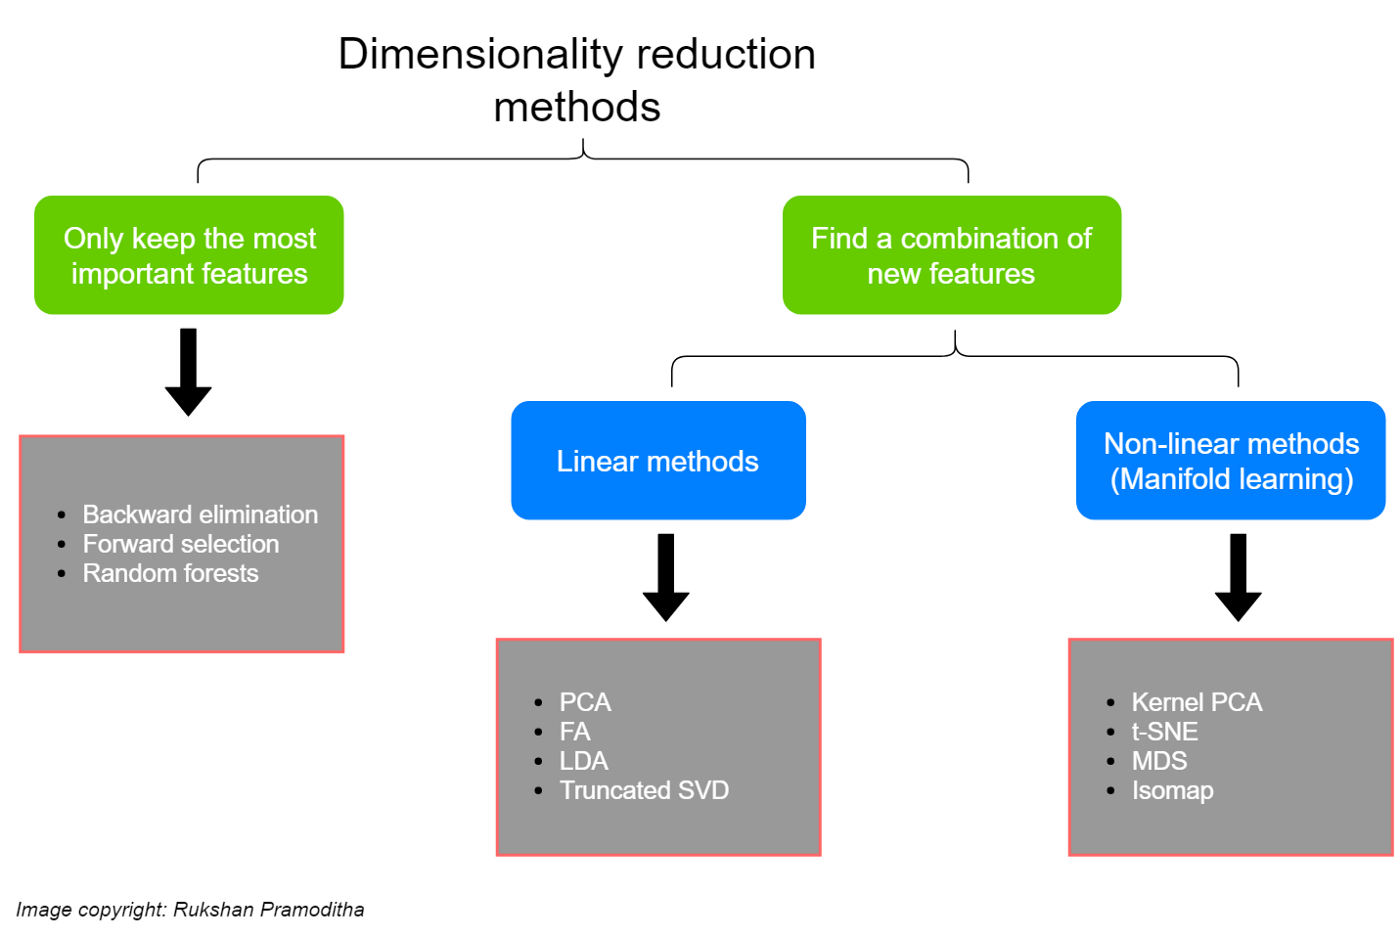
\includegraphics[scale=0.65]{figs/DR.png}
    \caption{Dimensionality Reduction methods}
    \label{fig:dim-reduction}
\end{figure}\newpage
    \hypertarget{principal-component-analysis-pca}{%
\subsubsection{Principal Component Analysis
(PCA)}\label{principal-component-analysis-pca}}

The first dimension reduction method that we're going to use is the
\emph{Principal Component Analysis (PCA)}. Principal component analysis
is used to extract the important information from a multivariate data
table and to express this information as a set of few new variables
called principal components. PCA assumes that the directions with the
largest variances are the most \textbf{important} while the amount of
variance retained by each principal component is measured by the
\textbf{eigenvalue}.\\
We will use the \texttt{prcomp()} method to obtain the \emph{PCA} and
then plot it:

    \begin{tcolorbox}[breakable, size=fbox, boxrule=1pt, pad at break*=1mm,colback=cellbackground, colframe=cellborder]
\prompt{In}{incolor}{9}{\boxspacing}
\begin{Verbatim}[commandchars=\\\{\}]
\PY{n}{pc} \PY{o}{\PYZlt{}\PYZhy{}} \PY{n+nf}{prcomp}\PY{p}{(}\PY{n}{ex}\PY{p}{)}
\PY{n+nf}{get\PYZus{}eigenvalue}\PY{p}{(}\PY{n}{pc}\PY{p}{)}\PY{p}{[}\PY{l+m}{1}\PY{o}{:}\PY{l+m}{5}\PY{p}{,} \PY{p}{]}
\end{Verbatim}
\end{tcolorbox}

    A data.frame: 5 × 3
\begin{tabular}{r|lll}
  & eigenvalue & variance.percent & cumulative.variance.percent\\
  & <dbl> & <dbl> & <dbl>\\
\hline
	Dim.1 & 299.598423 & 87.2509394 & 87.25094\\
	Dim.2 &  12.643203 &  3.6820333 & 90.93297\\
	Dim.3 &   6.430822 &  1.8728244 & 92.80580\\
	Dim.4 &   5.144998 &  1.4983587 & 94.30416\\
	Dim.5 &   3.140644 &  0.9146382 & 95.21879\\
\end{tabular}


    
    As you can see, about \(90.93%
\) of the variance is retained by the first two \emph{principal
components}.\\
Before going further, let's first plot the data according to \(PC1\) and
\(PC2\):

    \begin{tcolorbox}[breakable, size=fbox, boxrule=1pt, pad at break*=1mm,colback=cellbackground, colframe=cellborder]
\prompt{In}{incolor}{10}{\boxspacing}
\begin{Verbatim}[commandchars=\\\{\}]
\PY{n+nf}{options}\PY{p}{(}\PY{n}{repr.plot.width}\PY{o}{=}\PY{l+m}{15}\PY{p}{,} \PY{n}{repr.plot.height}\PY{o}{=}\PY{l+m}{6}\PY{p}{)}
\PY{n+nf}{par}\PY{p}{(}\PY{n}{mfrow} \PY{o}{=} \PY{n+nf}{c}\PY{p}{(}\PY{l+m}{1}\PY{p}{,} \PY{l+m}{2}\PY{p}{)}\PY{p}{)}
\PY{n}{p1} \PY{o}{\PYZlt{}\PYZhy{}} \PY{n+nf}{plot}\PY{p}{(}\PY{n}{pc}\PY{p}{)}
\PY{n}{p2} \PY{o}{\PYZlt{}\PYZhy{}} \PY{n+nf}{plot}\PY{p}{(}\PY{n}{pc}\PY{o}{\PYZdl{}}\PY{n}{x}\PY{p}{[}\PY{p}{,} \PY{l+m}{1}\PY{o}{:}\PY{l+m}{2}\PY{p}{]}\PY{p}{,} \PY{n}{las} \PY{o}{=} \PY{l+m}{2}\PY{p}{)}
\end{Verbatim}
\end{tcolorbox}

    \begin{center}
    \adjustimage{max size={0.9\linewidth}{0.9\paperheight}}{notebook_files/notebook_29_0.png}
    \end{center}
    { \hspace*{\fill} \\}
    
    The problem is, \(PC1\) seems to present a misleading variance in the
data points, acquired probably by the uninteresting expression
differences between genes which often expressed (e.g.~housekeeping
genes) and those expressed rarely.
\newpage
    To overcome this problem, we are going to center\footnote{Subtracting
  columns mean from their corresponding columns.} our data columns using
the \texttt{scale()} method:

    \begin{tcolorbox}[breakable, size=fbox, boxrule=1pt, pad at break*=1mm,colback=cellbackground, colframe=cellborder]
\prompt{In}{incolor}{11}{\boxspacing}
\begin{Verbatim}[commandchars=\\\{\}]
\PY{n}{ex.scale} \PY{o}{\PYZlt{}\PYZhy{}} \PY{n+nf}{t}\PY{p}{(}\PY{n+nf}{scale}\PY{p}{(}\PY{n+nf}{t}\PY{p}{(}\PY{n}{ex}\PY{p}{)}\PY{p}{,} \PY{n}{scale} \PY{o}{=} \PY{n+nb+bp}{F}\PY{p}{)}\PY{p}{)}
\PY{n}{pc} \PY{o}{\PYZlt{}\PYZhy{}} \PY{n+nf}{prcomp}\PY{p}{(}\PY{n}{ex.scale}\PY{p}{)}
\PY{n+nf}{get\PYZus{}eigenvalue}\PY{p}{(}\PY{n}{pc}\PY{p}{)}\PY{p}{[}\PY{l+m}{1}\PY{o}{:}\PY{l+m}{5}\PY{p}{,} \PY{p}{]}
\end{Verbatim}
\end{tcolorbox}

    A data.frame: 5 × 3
\begin{tabular}{r|lll}
  & eigenvalue & variance.percent & cumulative.variance.percent\\
  & <dbl> & <dbl> & <dbl>\\
\hline
	Dim.1 & 12.698222 & 28.876999 & 28.87700\\
	Dim.2 &  6.434864 & 14.633510 & 43.51051\\
	Dim.3 &  5.211775 & 11.852086 & 55.36259\\
	Dim.4 &  3.142359 &  7.146032 & 62.50863\\
	Dim.5 &  1.972313 &  4.485232 & 66.99386\\
\end{tabular}


    
    

    \begin{tcolorbox}[breakable, size=fbox, boxrule=1pt, pad at break*=1mm,colback=cellbackground, colframe=cellborder]
\prompt{In}{incolor}{12}{\boxspacing}
\begin{Verbatim}[commandchars=\\\{\}]
\PY{n+nf}{options}\PY{p}{(}\PY{n}{repr.plot.width}\PY{o}{=}\PY{l+m}{15}\PY{p}{,} \PY{n}{repr.plot.height}\PY{o}{=}\PY{l+m}{6}\PY{p}{)}
\PY{n+nf}{par}\PY{p}{(}\PY{n}{mfrow} \PY{o}{=} \PY{n+nf}{c}\PY{p}{(}\PY{l+m}{1}\PY{p}{,} \PY{l+m}{2}\PY{p}{)}\PY{p}{)}
\PY{n+nf}{plot}\PY{p}{(}\PY{n}{pc}\PY{p}{)}
\PY{n+nf}{plot}\PY{p}{(}\PY{n}{pc}\PY{o}{\PYZdl{}}\PY{n}{x}\PY{p}{[}\PY{p}{,} \PY{l+m}{1}\PY{o}{:}\PY{l+m}{2}\PY{p}{]}\PY{p}{)}
\end{Verbatim}
\end{tcolorbox}

    \begin{center}
    \adjustimage{max size={0.9\linewidth}{0.9\paperheight}}{notebook_files/notebook_35_0.png}
    \end{center}
    { \hspace*{\fill} \\}
    
    As you can see, now other components are contributing as well.
\newpage
    We can also plot the \emph{PCA} results according to the
\emph{variables}(which are the samples in this case) instead of the
\emph{individuals}(which are the genes in this case) to demonstrate
different sample groups and their correlation:

    \begin{tcolorbox}[breakable, size=fbox, boxrule=1pt, pad at break*=1mm,colback=cellbackground, colframe=cellborder]
\prompt{In}{incolor}{13}{\boxspacing}
\begin{Verbatim}[commandchars=\\\{\}]
\PY{n+nf}{options}\PY{p}{(}\PY{n}{repr.plot.width}\PY{o}{=}\PY{l+m}{20}\PY{p}{,} \PY{n}{repr.plot.height}\PY{o}{=}\PY{l+m}{8}\PY{p}{)}

\PY{n}{pcr} \PY{o}{\PYZlt{}\PYZhy{}} \PY{n+nf}{data.frame}\PY{p}{(}\PY{n}{pc}\PY{o}{\PYZdl{}}\PY{n}{rotation}\PY{p}{[}\PY{p}{,} \PY{l+m}{1}\PY{o}{:}\PY{l+m}{3}\PY{p}{]}\PY{p}{,} \PY{n}{Group}\PY{o}{=}\PY{n}{gs}\PY{p}{)}
\PY{n}{pca.plot1} \PY{o}{\PYZlt{}\PYZhy{}} \PY{n+nf}{ggplot}\PY{p}{(}\PY{n}{pcr}\PY{p}{,} 
                \PY{n+nf}{aes}\PY{p}{(}\PY{n}{x} \PY{o}{=} \PY{n}{PC1}\PY{p}{,} 
                    \PY{n}{y} \PY{o}{=} \PY{n}{PC2}\PY{p}{,} 
                    \PY{n}{color} \PY{o}{=} \PY{n}{Group}\PY{p}{)}\PY{p}{)} \PY{o}{+} \PY{n+nf}{geom\PYZus{}point}\PY{p}{(}\PY{n}{size}\PY{o}{=}\PY{l+m}{2.5}\PY{p}{)} \PY{o}{+} \PY{n+nf}{theme\PYZus{}gray}\PY{p}{(}\PY{p}{)}

\PY{n}{pca.plot2} \PY{o}{\PYZlt{}\PYZhy{}} \PY{n+nf}{fviz\PYZus{}pca\PYZus{}var}\PY{p}{(}\PY{n+nf}{PCA}\PY{p}{(}\PY{n}{ex.scale}\PY{p}{,} \PY{n}{graph} \PY{o}{=} \PY{k+kc}{FALSE}\PY{p}{)}\PY{p}{,} 
                      \PY{n}{col.var} \PY{o}{=} \PY{n}{gs}\PY{p}{,}
                      \PY{n}{legend.title} \PY{o}{=} \PY{l+s}{\PYZdq{}}\PY{l+s}{Group\PYZdq{}}\PY{p}{)}

\PY{n+nf}{ggarrange}\PY{p}{(}\PY{n}{pca.plot1}\PY{p}{,} \PY{k+kc}{NULL}\PY{p}{,} \PY{n}{pca.plot2}\PY{p}{,}
         \PY{n}{widths} \PY{o}{=} \PY{n+nf}{c}\PY{p}{(}\PY{l+m}{3}\PY{p}{,} \PY{l+m}{0.1}\PY{p}{,} \PY{l+m}{2}\PY{p}{)}\PY{p}{,}
         \PY{n}{labels} \PY{o}{=} \PY{n+nf}{c}\PY{p}{(}\PY{l+s}{\PYZsq{}}\PY{l+s}{A\PYZsq{}}\PY{p}{,} \PY{l+s}{\PYZsq{}}\PY{l+s}{\PYZsq{}}\PY{p}{,} \PY{l+s}{\PYZsq{}}\PY{l+s}{B\PYZsq{}}\PY{p}{)}\PY{p}{,}
         \PY{n}{ncol} \PY{o}{=} \PY{l+m}{3}\PY{p}{,}
         \PY{n}{nrow} \PY{o}{=} \PY{l+m}{1}\PY{p}{)}
\end{Verbatim}
\end{tcolorbox}

    \begin{center}
    \adjustimage{max size={0.9\linewidth}{0.9\paperheight}}{notebook_files/notebook_39_0.png}
    \end{center}
    { \hspace*{\fill} \\}
    
    About the figure \emph{B}:

\begin{itemize}
\tightlist
\item
  Positively correlated variables are grouped together.
\item
  Negatively correlated variables are positioned on opposite sides of
  the plot origin (opposed quadrants).
\end{itemize}
\newpage
    \hypertarget{t-distributed-stochastic-neighbor-embedding-tsne}{%
\subsubsection{t-distributed stochastic neighbor embedding
(tSNE)}\label{t-distributed-stochastic-neighbor-embedding-tsne}}

The next \emph{dimension reduction} algorithm that we're going to try is
the \emph{tSNE} which as mentioned in \hyperref[fig-1]{figure 1}, is a
\textbf{non-linear algorithm}. Non-linearity means that it's capable of
separating data which can't be separated by a straight line, unlike the
linear algorithms(e.g.~\emph{PCA}).

We're going to use the \texttt{Rtsne()} method from the \texttt{Rtsne}
package, to calculate the \emph{tSNE} of our expression matrix. One
parameter that we need to pass to the \texttt{Rtsne()} method is the
\textbf{\texttt{perplexity}}. A perplexity is more or less a target
number of neighbors for our central point. Basically, the higher the
perplexity is, the higher the variance value.\footnote{https://towardsdatascience.com/t-sne-clearly-explained-d84c537f53a}

So we will calculate the \emph{tSNE} for 3 \texttt{perplexity} values of
\(3, 5, 7, 10, 15\) and \(20\). After plotting the result, we can choose
the best value based on how well it separated the group clusters:

    \begin{tcolorbox}[breakable, size=fbox, boxrule=1pt, pad at break*=1mm,colback=cellbackground, colframe=cellborder]
\prompt{In}{incolor}{14}{\boxspacing}
\begin{Verbatim}[commandchars=\\\{\}]
\PY{n}{tsne\PYZus{}results} \PY{o}{\PYZlt{}\PYZhy{}} \PY{n+nf}{list}\PY{p}{(}\PY{n+nf}{Rtsne}\PY{p}{(}\PY{n+nf}{t}\PY{p}{(}\PY{n}{ex}\PY{p}{)}\PY{p}{,} \PY{n}{perplexity}\PY{o}{=}\PY{l+m}{3}\PY{p}{,} \PY{n}{check\PYZus{}duplicates} \PY{o}{=} \PY{k+kc}{FALSE}\PY{p}{)}\PY{p}{,}
                     \PY{n+nf}{Rtsne}\PY{p}{(}\PY{n+nf}{t}\PY{p}{(}\PY{n}{ex}\PY{p}{)}\PY{p}{,} \PY{n}{perplexity}\PY{o}{=}\PY{l+m}{5}\PY{p}{,} \PY{n}{check\PYZus{}duplicates} \PY{o}{=} \PY{k+kc}{FALSE}\PY{p}{)}\PY{p}{,}
                     \PY{n+nf}{Rtsne}\PY{p}{(}\PY{n+nf}{t}\PY{p}{(}\PY{n}{ex}\PY{p}{)}\PY{p}{,} \PY{n}{perplexity}\PY{o}{=}\PY{l+m}{7}\PY{p}{,} \PY{n}{check\PYZus{}duplicates} \PY{o}{=} \PY{k+kc}{FALSE}\PY{p}{)}\PY{p}{,}
                     \PY{n+nf}{Rtsne}\PY{p}{(}\PY{n+nf}{t}\PY{p}{(}\PY{n}{ex}\PY{p}{)}\PY{p}{,} \PY{n}{perplexity}\PY{o}{=}\PY{l+m}{10}\PY{p}{,} \PY{n}{check\PYZus{}duplicates} \PY{o}{=} \PY{k+kc}{FALSE}\PY{p}{)}\PY{p}{,}
                     \PY{n+nf}{Rtsne}\PY{p}{(}\PY{n+nf}{t}\PY{p}{(}\PY{n}{ex}\PY{p}{)}\PY{p}{,} \PY{n}{perplexity}\PY{o}{=}\PY{l+m}{15}\PY{p}{,} \PY{n}{check\PYZus{}duplicates} \PY{o}{=} \PY{k+kc}{FALSE}\PY{p}{)}\PY{p}{,}
                     \PY{n+nf}{Rtsne}\PY{p}{(}\PY{n+nf}{t}\PY{p}{(}\PY{n}{ex}\PY{p}{)}\PY{p}{,} \PY{n}{perplexity}\PY{o}{=}\PY{l+m}{20}\PY{p}{,} \PY{n}{check\PYZus{}duplicates} \PY{o}{=} \PY{k+kc}{FALSE}\PY{p}{)}\PY{p}{)}

\PY{n+nf}{options}\PY{p}{(}\PY{n}{repr.plot.width}\PY{o}{=}\PY{l+m}{16}\PY{p}{,} \PY{n}{repr.plot.height}\PY{o}{=}\PY{l+m}{14}\PY{p}{)}
\PY{n}{tsne.plots.list} \PY{o}{\PYZlt{}\PYZhy{}} \PY{n+nf}{list}\PY{p}{(}\PY{p}{)}

\PY{n+nf}{for}\PY{p}{(}\PY{n}{i} \PY{n}{in} \PY{n+nf}{seq\PYZus{}along}\PY{p}{(}\PY{n}{tsne\PYZus{}results}\PY{p}{)}\PY{p}{)} \PY{p}{\PYZob{}}
  \PY{n}{tsne} \PY{o}{\PYZlt{}\PYZhy{}} \PY{n+nf}{data.frame}\PY{p}{(}\PY{n}{tsne\PYZus{}results}\PY{p}{[[}\PY{n}{i}\PY{p}{]]}\PY{o}{\PYZdl{}}\PY{n}{Y}\PY{p}{[}\PY{p}{,} \PY{l+m}{1}\PY{o}{:}\PY{l+m}{2}\PY{p}{]}\PY{p}{,} \PY{n}{Group}\PY{o}{=}\PY{n}{gs}\PY{p}{)}
  \PY{n}{tsne.plots.list}\PY{p}{[[}\PY{n}{i}\PY{p}{]]} \PY{o}{\PYZlt{}\PYZhy{}} \PY{n+nf}{ggplot}\PY{p}{(}\PY{n}{tsne}\PY{p}{,} \PY{n+nf}{aes}\PY{p}{(}\PY{n}{X1}\PY{p}{,} \PY{n}{X2}\PY{p}{,} \PY{n}{color} \PY{o}{=} \PY{n}{Group}\PY{p}{)}\PY{p}{)} \PY{o}{+} \PY{n+nf}{geom\PYZus{}point}\PY{p}{(}\PY{n}{size}\PY{o}{=}\PY{l+m}{2}\PY{p}{)} \PY{o}{+} \PY{n+nf}{theme\PYZus{}gray}\PY{p}{(}\PY{p}{)}
\PY{p}{\PYZcb{}}
\PY{n}{ggarr} \PY{o}{\PYZlt{}\PYZhy{}} \PY{n+nf}{ggarrange}\PY{p}{(}\PY{n}{plotlist} \PY{o}{=} \PY{n}{tsne.plots.list}\PY{p}{,} 
                   \PY{n}{ncol} \PY{o}{=} \PY{l+m}{2}\PY{p}{,} 
                   \PY{n}{nrow} \PY{o}{=} \PY{l+m}{3}\PY{p}{,}
                  \PY{n}{labels} \PY{o}{=} \PY{n+nf}{c}\PY{p}{(}\PY{l+m}{3}\PY{p}{,} \PY{l+m}{5}\PY{p}{,} \PY{l+m}{7}\PY{p}{,} \PY{l+m}{10}\PY{p}{,} \PY{l+m}{15}\PY{p}{,} \PY{l+m}{20}\PY{p}{)}\PY{p}{)}
\PY{n+nf}{annotate\PYZus{}figure}\PY{p}{(}\PY{n}{ggarr}\PY{p}{,}
               \PY{n}{bottom} \PY{o}{=} \PY{n+nf}{text\PYZus{}grob}\PY{p}{(}\PY{l+s}{\PYZdq{}}\PY{l+s}{tSNE with the perplexity around 5\PYZhy{}10 is sufficient.\PYZdq{}}\PY{p}{,}
                                  \PY{n}{hjust} \PY{o}{=} \PY{l+m}{1}\PY{p}{,}
                                  \PY{n}{x} \PY{o}{=} \PY{l+m}{1}\PY{p}{,}
                                  \PY{n}{face} \PY{o}{=} \PY{l+s}{\PYZdq{}}\PY{l+s}{italic\PYZdq{}}\PY{p}{,}
                                  \PY{n}{size} \PY{o}{=} \PY{l+m}{14}\PY{p}{)}
               \PY{p}{)}
\end{Verbatim}
\end{tcolorbox}

    \begin{center}
    \adjustimage{max size={0.9\linewidth}{0.9\paperheight}}{notebook_files/notebook_43_0.png}
    \end{center}
    { \hspace*{\fill} \\}
    
    According to the plots, \emph{tSNE} with the \texttt{perplexity} in a
range \([5, 10]\) was almost successful to separate different groups of
samples \textbf{except for the \emph{AML}, \emph{CD34+}, and
\emph{Monocytes}} which brings this idea to mind that expressions in
these groups were highly similar/correlated.
\newpage
    \hypertarget{multidimensional-scaling-mds}{%
\subsubsection{Multidimensional scaling
(MDS)}\label{multidimensional-scaling-mds}}

\emph{MDS} returns an optimal solution to represent the data in a
lower-dimensional space, where the number of dimensions \(k\) is
pre-specified by the analyst. For example, choosing \(k = 2\) optimizes
the object locations for a two-dimensional scatter plot.

The input data for MDS is a dissimilarity matrix representing the
distances between pairs of objects. So first we will compute the
distance matrix using the \texttt{dist()} method:

    \begin{tcolorbox}[breakable, size=fbox, boxrule=1pt, pad at break*=1mm,colback=cellbackground, colframe=cellborder]
\prompt{In}{incolor}{15}{\boxspacing}
\begin{Verbatim}[commandchars=\\\{\}]
\PY{n}{ex\PYZus{}dist} \PY{o}{\PYZlt{}\PYZhy{}} \PY{n+nf}{dist}\PY{p}{(}\PY{n+nf}{t}\PY{p}{(}\PY{n}{ex.scale}\PY{p}{)}\PY{p}{)}
\end{Verbatim}
\end{tcolorbox}

    Now we can pass the \texttt{ex\_dist} to the \texttt{cmdscale} from the
\texttt{stats} package to compute the \emph{mds} result:

    \begin{tcolorbox}[breakable, size=fbox, boxrule=1pt, pad at break*=1mm,colback=cellbackground, colframe=cellborder]
\prompt{In}{incolor}{16}{\boxspacing}
\begin{Verbatim}[commandchars=\\\{\}]
\PY{n+nf}{options}\PY{p}{(}\PY{n}{repr.plot.width}\PY{o}{=}\PY{l+m}{6}\PY{p}{,} \PY{n}{repr.plot.height}\PY{o}{=}\PY{l+m}{4}\PY{p}{)}

\PY{n}{mds\PYZus{}result} \PY{o}{\PYZlt{}\PYZhy{}} \PY{n+nf}{cmdscale}\PY{p}{(}\PY{n}{ex\PYZus{}dist}\PY{p}{,} \PY{n}{eig}\PY{o}{=}\PY{k+kc}{TRUE}\PY{p}{,} \PY{n}{k}\PY{o}{=}\PY{l+m}{2}\PY{p}{)}
\PY{n}{mds\PYZus{}df} \PY{o}{\PYZlt{}\PYZhy{}} \PY{n+nf}{data.frame}\PY{p}{(}\PY{n}{mds\PYZus{}result}\PY{o}{\PYZdl{}}\PY{n}{points}\PY{p}{[}\PY{p}{,}\PY{l+m}{1}\PY{o}{:}\PY{l+m}{2}\PY{p}{]}\PY{p}{,} \PY{n}{Group}\PY{o}{=}\PY{n}{gs}\PY{p}{)}
\PY{n}{mds.plot} \PY{o}{\PYZlt{}\PYZhy{}} \PY{n+nf}{ggplot}\PY{p}{(}\PY{n}{mds\PYZus{}df}\PY{p}{,} \PY{n+nf}{aes}\PY{p}{(}\PY{n}{X1}\PY{p}{,}\PY{n}{X2}\PY{p}{,} \PY{n}{color} \PY{o}{=} \PY{n}{Group}\PY{p}{)}\PY{p}{)} \PY{o}{+} \PY{n+nf}{geom\PYZus{}point}\PY{p}{(}\PY{n}{size}\PY{o}{=}\PY{l+m}{2.5}\PY{p}{)} \PY{o}{+} \PY{n+nf}{theme\PYZus{}gray}\PY{p}{(}\PY{p}{)}
\PY{n}{mds.plot}
\end{Verbatim}
\end{tcolorbox}

    \begin{center}
    \adjustimage{max size={0.9\linewidth}{0.9\paperheight}}{notebook_files/notebook_49_0.png}
    \end{center}
    { \hspace*{\fill} \\}
    \newpage
    \hypertarget{pca-vs.-tsne-vs.-mds}{%
\subsubsection{PCA vs.~tSNE vs.~MDS}\label{pca-vs.-tsne-vs.-mds}}

To compare the results of these 3 methods, we will plot their results
one more time to make it easier for comparing:

    \begin{tcolorbox}[breakable, size=fbox, boxrule=1pt, pad at break*=1mm,colback=cellbackground, colframe=cellborder]
\prompt{In}{incolor}{17}{\boxspacing}
\begin{Verbatim}[commandchars=\\\{\}]
\PY{n+nf}{options}\PY{p}{(}\PY{n}{repr.plot.width}\PY{o}{=}\PY{l+m}{16}\PY{p}{,} \PY{n}{repr.plot.height}\PY{o}{=}\PY{l+m}{10}\PY{p}{)}
\PY{n+nf}{ggarrange}\PY{p}{(}\PY{n}{pca.plot1}\PY{p}{,} \PY{n}{tsne.plots.list}\PY{p}{[[}\PY{l+m}{4}\PY{p}{]]}\PY{p}{,} \PY{n}{mds.plot}\PY{p}{,}
          \PY{n}{ncol} \PY{o}{=} \PY{l+m}{2}\PY{p}{,}
          \PY{n}{nrow} \PY{o}{=} \PY{l+m}{2}\PY{p}{,}
          \PY{n}{labels} \PY{o}{=} \PY{n+nf}{c}\PY{p}{(}\PY{l+s}{\PYZsq{}}\PY{l+s}{PCA\PYZsq{}}\PY{p}{,} \PY{l+s}{\PYZsq{}}\PY{l+s}{tSNE\PYZsq{}}\PY{p}{,} \PY{l+s}{\PYZsq{}}\PY{l+s}{MDS\PYZsq{}}\PY{p}{)}\PY{p}{)}
\end{Verbatim}
\end{tcolorbox}

    \begin{center}
    \adjustimage{max size={0.9\linewidth}{0.9\paperheight}}{notebook_files/notebook_52_0.png}
    \end{center}
    { \hspace*{\fill} \\}
    
    According to plots, we believe that the \textbf{\emph{tSNE}} was able to
separate groups of samples more precisely.
\newpage
    \hypertarget{correlation-between-samples}{%
\subsection{Correlation between
samples}\label{correlation-between-samples}}

Heat map shows correlations between different samples. For example each
group has high corealation with itself that is determined by red color
or \emph{Granulocytes} have a low correlation with \emph{B-cells} and
\emph{T-cells} which is determined by blue color.

According to the heatmap, \textbf{\emph{AML}} has a high correlation
with \textbf{\emph{CD34+}} and \textbf{\emph{Monocytes}} which makes
these 2 groups, proper candidates to check whether there are any
significant expression differences between their genes and the
\emph{AML} ones.

    \begin{tcolorbox}[breakable, size=fbox, boxrule=1pt, pad at break*=1mm,colback=cellbackground, colframe=cellborder]
\prompt{In}{incolor}{18}{\boxspacing}
\begin{Verbatim}[commandchars=\\\{\}]
\PY{n+nf}{options}\PY{p}{(}\PY{n}{repr.plot.width}\PY{o}{=}\PY{l+m}{10}\PY{p}{,} \PY{n}{repr.plot.height}\PY{o}{=}\PY{l+m}{10}\PY{p}{)}
\PY{n+nf}{pheatmap}\PY{p}{(}\PY{n+nf}{cor}\PY{p}{(}\PY{n}{ex}\PY{p}{)}\PY{p}{,}
         \PY{n}{labels\PYZus{}row} \PY{o}{=} \PY{n}{gs}\PY{p}{,}
         \PY{n}{labels\PYZus{}col} \PY{o}{=} \PY{n}{gs}\PY{p}{,}
         \PY{n}{border\PYZus{}color} \PY{o}{=} \PY{k+kc}{NA}\PY{p}{,}\PY{p}{)}
\end{Verbatim}
\end{tcolorbox}

    \begin{center}
    \adjustimage{max size={0.9\linewidth}{0.9\paperheight}}{notebook_files/notebook_56_0.png}
    \end{center}
    { \hspace*{\fill} \\}
    
    \hypertarget{differential-expression-analysis}{%
\section{Differential expression
analysis}\label{differential-expression-analysis}}

    \hypertarget{fitting-a-linear-model-to-the-data}{%
\subsection{Fitting a linear model to the
data}\label{fitting-a-linear-model-to-the-data}}

creating a \emph{design matrix} which simply demonstrates which group,
each sample belongs to:

    \begin{tcolorbox}[breakable, size=fbox, boxrule=1pt, pad at break*=1mm,colback=cellbackground, colframe=cellborder]
\prompt{In}{incolor}{19}{\boxspacing}
\begin{Verbatim}[commandchars=\\\{\}]
\PY{n}{design} \PY{o}{\PYZlt{}\PYZhy{}} \PY{n+nf}{model.matrix}\PY{p}{(}\PY{o}{\PYZti{}} \PY{n}{group} \PY{o}{+} \PY{l+m}{0}\PY{p}{,} \PY{n}{gset}\PY{p}{)}
\PY{n+nf}{colnames}\PY{p}{(}\PY{n}{design}\PY{p}{)} \PY{o}{\PYZlt{}\PYZhy{}} \PY{n+nf}{levels}\PY{p}{(}\PY{n}{gs}\PY{p}{)}
\end{Verbatim}
\end{tcolorbox}

    \begin{tcolorbox}[breakable, size=fbox, boxrule=1pt, pad at break*=1mm,colback=cellbackground, colframe=cellborder]
\prompt{In}{incolor}{20}{\boxspacing}
\begin{Verbatim}[commandchars=\\\{\}]
\PY{n+nf}{head}\PY{p}{(}\PY{n}{design}\PY{p}{)}
\end{Verbatim}
\end{tcolorbox}

    A matrix: 6 × 6 of type dbl
\begin{tabular}{r|llllll}
  & AML & Granulocytes & B.Cells & T.Cells & Monocytes & CD34\\
\hline
	GSM1180750 & 1 & 0 & 0 & 0 & 0 & 0\\
	GSM1180751 & 1 & 0 & 0 & 0 & 0 & 0\\
	GSM1180752 & 1 & 0 & 0 & 0 & 0 & 0\\
	GSM1180753 & 1 & 0 & 0 & 0 & 0 & 0\\
	GSM1180754 & 1 & 0 & 0 & 0 & 0 & 0\\
	GSM1180755 & 1 & 0 & 0 & 0 & 0 & 0\\
\end{tabular}


    
    Now we try to fit a simple linear model to the gene expressions:

    \begin{tcolorbox}[breakable, size=fbox, boxrule=1pt, pad at break*=1mm,colback=cellbackground, colframe=cellborder]
\prompt{In}{incolor}{21}{\boxspacing}
\begin{Verbatim}[commandchars=\\\{\}]
\PY{n}{fit} \PY{o}{\PYZlt{}\PYZhy{}} \PY{n+nf}{lmFit}\PY{p}{(}\PY{n}{gset}\PY{p}{,} \PY{n}{design}\PY{p}{)}
\end{Verbatim}
\end{tcolorbox}

    Comparisons between groups(log fold-changes) are obtained as contrasts
of these fitted linear models. Here we choose the \textbf{\emph{AML}}
and the \textbf{\emph{CD34}} groups to compare:

    \begin{tcolorbox}[breakable, size=fbox, boxrule=1pt, pad at break*=1mm,colback=cellbackground, colframe=cellborder]
\prompt{In}{incolor}{22}{\boxspacing}
\begin{Verbatim}[commandchars=\\\{\}]
\PY{n}{cont.matrix} \PY{o}{\PYZlt{}\PYZhy{}} \PY{n+nf}{makeContrasts}\PY{p}{(}\PY{n}{AML}\PY{o}{\PYZhy{}}\PY{n}{CD34}\PY{p}{,} \PY{n}{levels}\PY{o}{=}\PY{n}{design}\PY{p}{)}
\end{Verbatim}
\end{tcolorbox}

    now we use the \texttt{contrasts.fit()} to compute estimated
coefficients and standard errors for the \textbf{\emph{AML-CD34}}
contrasts. It actually estimates contrast for each gene:

    \begin{tcolorbox}[breakable, size=fbox, boxrule=1pt, pad at break*=1mm,colback=cellbackground, colframe=cellborder]
\prompt{In}{incolor}{23}{\boxspacing}
\begin{Verbatim}[commandchars=\\\{\}]
\PY{n}{fit2} \PY{o}{\PYZlt{}\PYZhy{}} \PY{n+nf}{contrasts.fit}\PY{p}{(}\PY{n}{fit}\PY{p}{,} \PY{n}{cont.matrix}\PY{p}{)}
\end{Verbatim}
\end{tcolorbox}

    Empirical Bayes smoothing of standard errors(shrinks standard errors
that are much larger or smaller than those from other genes towards the
average standard error):

    \begin{tcolorbox}[breakable, size=fbox, boxrule=1pt, pad at break*=1mm,colback=cellbackground, colframe=cellborder]
\prompt{In}{incolor}{24}{\boxspacing}
\begin{Verbatim}[commandchars=\\\{\}]
\PY{n}{fit2} \PY{o}{\PYZlt{}\PYZhy{}} \PY{n+nf}{eBayes}\PY{p}{(}\PY{n}{fit2}\PY{p}{,} \PY{l+m}{0.01}\PY{p}{)}
\end{Verbatim}
\end{tcolorbox}
\newpage
    \hypertarget{top-ranked-genes}{%
\subsection{Top-ranked genes}\label{top-ranked-genes}}

Now we will extract a table of the top-ranked genes from our linear
model \texttt{fit2}:

    \begin{tcolorbox}[breakable, size=fbox, boxrule=1pt, pad at break*=1mm,colback=cellbackground, colframe=cellborder]
\prompt{In}{incolor}{25}{\boxspacing}
\begin{Verbatim}[commandchars=\\\{\}]
\PY{n}{tT} \PY{o}{\PYZlt{}\PYZhy{}} \PY{n+nf}{topTable}\PY{p}{(}\PY{n}{fit2}\PY{p}{,} \PY{n}{adjust}\PY{o}{=}\PY{l+s}{\PYZdq{}}\PY{l+s}{fdr\PYZdq{}}\PY{p}{,} \PY{n}{sort.by}\PY{o}{=}\PY{l+s}{\PYZdq{}}\PY{l+s}{B\PYZdq{}}\PY{p}{,} \PY{n}{number}\PY{o}{=}\PY{k+kc}{Inf}\PY{p}{)}
\PY{n}{tT} \PY{o}{\PYZlt{}\PYZhy{}} \PY{n+nf}{subset}\PY{p}{(}\PY{n}{tT}\PY{p}{,} \PY{n}{select}\PY{o}{=}\PY{n+nf}{c}\PY{p}{(}\PY{l+s}{\PYZdq{}}\PY{l+s}{Gene.symbol\PYZdq{}}\PY{p}{,}\PY{l+s}{\PYZdq{}}\PY{l+s}{Gene.ID\PYZdq{}}\PY{p}{,}\PY{l+s}{\PYZdq{}}\PY{l+s}{adj.P.Val\PYZdq{}}\PY{p}{,}\PY{l+s}{\PYZdq{}}\PY{l+s}{logFC\PYZdq{}}\PY{p}{)}\PY{p}{)}
\end{Verbatim}
\end{tcolorbox}

    As you can see below, \texttt{tT} consists of \(32321\) genes in the
rows and the columns are \emph{Gene.symbol}, \emph{Gene.ID},
\emph{adj.P.Val} and \emph{logFC}. Genes are sorted according to the
\textbf{\emph{B}} values by passing the \texttt{sort.by="B"} argument to
the \texttt{topTable()} mathod:

    \begin{tcolorbox}[breakable, size=fbox, boxrule=1pt, pad at break*=1mm,colback=cellbackground, colframe=cellborder]
\prompt{In}{incolor}{26}{\boxspacing}
\begin{Verbatim}[commandchars=\\\{\}]
\PY{n+nf}{print}\PY{p}{(}\PY{n+nf}{dim}\PY{p}{(}\PY{n}{tT}\PY{p}{)}\PY{p}{)}
\PY{n+nf}{head}\PY{p}{(}\PY{n}{tT}\PY{p}{)}
\end{Verbatim}
\end{tcolorbox}

    \begin{Verbatim}[commandchars=\\\{\}]
[1] 32321     4
    \end{Verbatim}

    A data.frame: 6 × 4
\begin{tabular}{r|llll}
  & Gene.symbol & Gene.ID & adj.P.Val & logFC\\
  & <chr> & <chr> & <dbl> & <dbl>\\
\hline
	8160088 & MPDZ   & 8777   & 2.565924e-36 & -3.670064\\
	8101284 & PRKG2  & 5593   & 5.887234e-30 & -5.874765\\
	7910915 & CHRM3  & 1131   & 3.200429e-28 & -4.378570\\
	8160168 & FREM1  & 158326 & 1.119567e-23 & -3.409825\\
	8121814 & NKAIN2 & 154215 & 5.166675e-23 & -4.673490\\
	8008588 & HLF    & 3131   & 2.786807e-20 & -4.140364\\
\end{tabular}


    
    We can save the resulting differential expression matrix in a file:

    \begin{tcolorbox}[breakable, size=fbox, boxrule=1pt, pad at break*=1mm,colback=cellbackground, colframe=cellborder]
\prompt{In}{incolor}{27}{\boxspacing}
\begin{Verbatim}[commandchars=\\\{\}]
\PY{n+nf}{write.table}\PY{p}{(}\PY{n}{tT}\PY{p}{,}
            \PY{n}{file}\PY{o}{=}\PY{l+s}{\PYZdq{}}\PY{l+s}{../Results/AML\PYZus{}CD34.txt\PYZdq{}}\PY{p}{,}
            \PY{n}{row.names}\PY{o}{=}\PY{n+nb+bp}{F}\PY{p}{,}
            \PY{n}{sep}\PY{o}{=}\PY{l+s}{\PYZdq{}}\PY{l+s}{\PYZbs{}t\PYZdq{}}\PY{p}{,}
            \PY{n}{quote}\PY{o}{=}\PY{n+nb+bp}{F}\PY{p}{)}
\end{Verbatim}
\end{tcolorbox}
\newpage
    \hypertarget{aml-up-genes}{%
\subsubsection{AML up genes}\label{aml-up-genes}}

Now it's the time to achieve a list of \textbf{\emph{AML-CD34}} genes
which highly expressed in the case of AML patients:

    \begin{tcolorbox}[breakable, size=fbox, boxrule=1pt, pad at break*=1mm,colback=cellbackground, colframe=cellborder]
\prompt{In}{incolor}{28}{\boxspacing}
\begin{Verbatim}[commandchars=\\\{\}]
\PY{n}{aml.up} \PY{o}{\PYZlt{}\PYZhy{}} \PY{n+nf}{subset}\PY{p}{(}\PY{n}{tT}\PY{p}{,} \PY{n}{logFC} \PY{o}{\PYZgt{}} \PY{l+m}{1} \PY{o}{\PYZam{}} \PY{n}{adj.P.Val} \PY{o}{\PYZlt{}} \PY{l+m}{0.05}\PY{p}{)}
\PY{n}{aml.up.genes} \PY{o}{\PYZlt{}\PYZhy{}} \PY{n+nf}{unique}\PY{p}{(}\PY{n+nf}{as.character}\PY{p}{(}\PY{n+nf}{strsplit2}\PY{p}{(}\PY{n}{aml.up}\PY{o}{\PYZdl{}}\PY{n}{Gene.symbol}\PY{p}{,} \PY{l+s}{\PYZsq{}}\PY{l+s}{///\PYZsq{}}\PY{p}{)}\PY{p}{)}\PY{p}{)}

\PY{n+nf}{write.table}\PY{p}{(}\PY{n}{aml.up.genes}\PY{p}{,}
            \PY{n}{file}\PY{o}{=}\PY{l+s}{\PYZdq{}}\PY{l+s}{../Results/AML\PYZus{}CD34\PYZus{}Up.txt\PYZdq{}}\PY{p}{,}
            \PY{n}{quote}\PY{o}{=}\PY{n+nb+bp}{F}\PY{p}{,}
            \PY{n}{col.names}\PY{o}{=}\PY{n+nb+bp}{F}\PY{p}{,}
            \PY{n}{row.names}\PY{o}{=}\PY{n+nb+bp}{F}\PY{p}{)}
\end{Verbatim}
\end{tcolorbox}

    \begin{tcolorbox}[breakable, size=fbox, boxrule=1pt, pad at break*=1mm,colback=cellbackground, colframe=cellborder]
\prompt{In}{incolor}{29}{\boxspacing}
\begin{Verbatim}[commandchars=\\\{\}]
\PY{n+nf}{head}\PY{p}{(}\PY{n+nf}{unique}\PY{p}{(}\PY{n}{aml.up}\PY{p}{)}\PY{p}{)}
\end{Verbatim}
\end{tcolorbox}

    A data.frame: 6 × 4
\begin{tabular}{r|llll}
  & Gene.symbol & Gene.ID & adj.P.Val & logFC\\
  & <chr> & <chr> & <dbl> & <dbl>\\
\hline
	8111739 & FYB         & 2533            & 7.381406e-13 & 4.382383\\
	8080487 & PRKCD       & 5580            & 1.411050e-12 & 2.972528\\
	8034420 & MAN2B1      & 4125            & 2.608491e-09 & 1.932052\\
	7973108 & ECRP///ECRP & 643332///643332 & 1.590050e-08 & 4.248503\\
	7907830 & QSOX1       & 5768            & 1.749850e-08 & 2.173438\\
	7970162 & ATP11A      & 23250           & 2.212408e-08 & 2.026483\\
\end{tabular}


    
    \hypertarget{aml-down-genes}{%
\subsubsection{AML down genes}\label{aml-down-genes}}

Then also a list of \textbf{\emph{AML-CD34}} genes which had a
low-expression:

    \begin{tcolorbox}[breakable, size=fbox, boxrule=1pt, pad at break*=1mm,colback=cellbackground, colframe=cellborder]
\prompt{In}{incolor}{30}{\boxspacing}
\begin{Verbatim}[commandchars=\\\{\}]
\PY{n}{aml.down} \PY{o}{\PYZlt{}\PYZhy{}} \PY{n+nf}{subset}\PY{p}{(}\PY{n}{tT}\PY{p}{,} \PY{n}{logFC} \PY{o}{\PYZlt{}} \PY{l+m}{\PYZhy{}1} \PY{o}{\PYZam{}} \PY{n}{adj.P.Val} \PY{o}{\PYZlt{}} \PY{l+m}{0.05}\PY{p}{)}
\PY{n}{aml.down.genes} \PY{o}{\PYZlt{}\PYZhy{}} \PY{n+nf}{unique}\PY{p}{(}\PY{n+nf}{as.character}\PY{p}{(}\PY{n+nf}{strsplit2}\PY{p}{(}\PY{n}{aml.down}\PY{o}{\PYZdl{}}\PY{n}{Gene.symbol}\PY{p}{,} \PY{l+s}{\PYZsq{}}\PY{l+s}{///\PYZsq{}}\PY{p}{)}\PY{p}{)}\PY{p}{)}

\PY{n+nf}{write.table}\PY{p}{(}\PY{n}{aml.down.genes}\PY{p}{,}
            \PY{n}{file}\PY{o}{=}\PY{l+s}{\PYZdq{}}\PY{l+s}{../Results/AML\PYZus{}CD34\PYZus{}Down.txt\PYZdq{}}\PY{p}{,}
            \PY{n}{quote}\PY{o}{=}\PY{n+nb+bp}{F}\PY{p}{,}
            \PY{n}{col.names}\PY{o}{=}\PY{n+nb+bp}{F}\PY{p}{,}
            \PY{n}{row.names}\PY{o}{=}\PY{n+nb+bp}{F}\PY{p}{)}
\end{Verbatim}
\end{tcolorbox}

    \begin{tcolorbox}[breakable, size=fbox, boxrule=1pt, pad at break*=1mm,colback=cellbackground, colframe=cellborder]
\prompt{In}{incolor}{31}{\boxspacing}
\begin{Verbatim}[commandchars=\\\{\}]
\PY{n+nf}{head}\PY{p}{(}\PY{n+nf}{unique}\PY{p}{(}\PY{n}{aml.down}\PY{p}{)}\PY{p}{)}
\end{Verbatim}
\end{tcolorbox}

    A data.frame: 6 × 4
\begin{tabular}{r|llll}
  & Gene.symbol & Gene.ID & adj.P.Val & logFC\\
  & <chr> & <chr> & <dbl> & <dbl>\\
\hline
	8160088 & MPDZ   & 8777   & 2.565924e-36 & -3.670064\\
	8101284 & PRKG2  & 5593   & 5.887234e-30 & -5.874765\\
	7910915 & CHRM3  & 1131   & 3.200429e-28 & -4.378570\\
	8160168 & FREM1  & 158326 & 1.119567e-23 & -3.409825\\
	8121814 & NKAIN2 & 154215 & 5.166675e-23 & -4.673490\\
	8008588 & HLF    & 3131   & 2.786807e-20 & -4.140364\\
\end{tabular}


    \newpage
    \hypertarget{transcription-analysis}{%
\subsection{Transcription Analysis}\label{transcription-analysis}}
\begin{figure}
  \begin{center}
      \begin{subfigure}{.5\textwidth}
          \adjustimage{width=1\linewidth, right}{figs/ChEA_2022_bar_graph.png}
          \caption{ChEA 2022}\label{fig:chea-2022}
      \end{subfigure}%
      \hspace*{.1in}
      \begin{subfigure}{.5\textwidth}
          \adjustimage{width=1\linewidth, left}{figs/ENCODE_and_ChEA_Consensus_TFs_from_ChIP-X_bar_graph.png}
          \caption{ENCODE and ChEA Consensus TFs from ChIP-X}\label{fig:encode-chea}
      \end{subfigure}
  \end{center}
\end{figure}
    \hypertarget{pathway-analysis}{%
\subsection{Pathway Analysis}\label{pathway-analysis}}
\begin{figure}
  \begin{center}
      \begin{subfigure}{.5\textwidth}
          \adjustimage{width=1\linewidth, right}{figs/Reactome_2022_bar_graph.png}
          \caption{Reactome 2022}\label{fig:reactome-2022}
      \end{subfigure}%
      \hspace*{.1in}
      \begin{subfigure}{.5\textwidth}
          \adjustimage{width=1\linewidth, left}{figs/KEGG_2021_Human_bar_graph.png}
          \caption{KEGG 2021}\label{fig:KEGG-2021}
      \end{subfigure}
      \hfill
  \end{center}
  \begin{subfigure}{.5\textwidth}
    \adjustimage{width=1\linewidth, left}{figs/WikiPathway_2021_Human_bar_graph.png}
    \caption{WikiPathway 2021}\label{fig:wikipathway-2021}
  \end{subfigure}
  \hspace*{.1in}
  \begin{subfigure}{.5\textwidth}
  \end{subfigure}
\end{figure}
    \hypertarget{gene-ontology-analysis}{%
\subsection{Gene Ontology Analysis}\label{gene-ontology-analysis}}
\begin{figure}
  \begin{center}
      \begin{subfigure}{.5\textwidth}
          \adjustimage{width=1\linewidth, right}{figs/GO_Biological_Process_2021_bar_graph.png}
          \caption{GO Biological Process 2021}\label{fig:go-bio-pro-2021}
      \end{subfigure}%
      \hspace*{.1in}
      \begin{subfigure}{.5\textwidth}
          \adjustimage{width=1\linewidth, left}{figs/GO_Cellular_Component_2021_bar_graph.png}
          \caption{GO Cellular Component 2021}\label{fig:go-cell-comp-2021}
      \end{subfigure}
      \hfill
  \end{center}
  \begin{subfigure}{.5\textwidth}
    \adjustimage{width=1\linewidth, left}{figs/GO_Molecular_Function_2021_bar_graph.png}
    \caption{GO Molecular Function 2021}\label{fig:go-mol-func-2021}
  \end{subfigure}
  \hspace*{.1in}
  \begin{subfigure}{.5\textwidth}
  \end{subfigure}
\end{figure}
    \hypertarget{validation}{%
\subsection{Validation}\label{validation}}

To validate our results, we will demonstrate some prior researches which
can confirm our results.

    \hypertarget{foxm1}{%
\subsubsection{FOXM1}\label{foxm1}}

FOXM1, a known transcription factor, promotes cell proliferation in a
variety of cancer cells. our study shows a critical role and mechanisms
of Foxm1 in MA9-LSCs, and indicates that FOXM1 is a potential
therapeutic target for selectively eliminating LSCs in MLL-rearranged
AML.\footnote{\href{https://www.nature.com/articles/s41467-020-14590-9}{FOXM1
  regulates leukemia stem cell quiescence and survival in MLL-rearranged
  AML}}

    \hypertarget{e2f4}{%
\subsubsection{E2F4}\label{e2f4}}

the experimental results showed that E2F4 was aberrantly overexpressed
in human AML patients and cell lines. Depletion of E2F4 inhibited the
proliferation, induced the differentiation and suppressed the growth of
AML cells in a nude mouse model. By contrast, overexpression of E2F4
promoted the proliferation and inhibited the differentiation of AML
cells in vitro.\footnote{\href{https://pubmed.ncbi.nlm.nih.gov/31943751/}{E2F4
  functions as a tumour suppressor in acute myeloid leukaemia via
  inhibition of the MAPK signalling pathway by binding to EZH2}}

    \hypertarget{t-cell-receptor}{%
\subsubsection{T Cell Receptor}\label{t-cell-receptor}}

In vitro studies show that coculture with AML cells and incubations with
AML plasma inhibit the proliferation of T cells. One proven mechanism of
T cell growth inhibition is the expression of AML surface receptors that
interact with T cells and alter their function. This includes leukocyte
immunoglobulin-like receptor B4 (LILRB4), an inhibitory immune
checkpoint receptor restrictively expressed on monocytic leukemic cells
(M4 and M5 subtypes).\footnote{\href{https://www.ncbi.nlm.nih.gov/pmc/articles/PMC8699747/}{The
  Role of T Cell Immunotherapy in Acute Myeloid Leukemia}}

    \hypertarget{phagosome}{%
\subsubsection{Phagosome}\label{phagosome}}

It is reported that phagosome pathway is the most optimal and common in
both Kasumi-1 and MV4-11 AML cell lines induced by differentiation
inducers, Trichostatin A and 5-Azacytidine (Asmaa et al.,
2020)\footnote{\href{https://www.frontiersin.org/articles/10.3389/fcell.2021.652972/full}{OGP46
  Induces Differentiation of Acute Myeloid Leukemia Cells via Different
  Optimal Signaling Pathways}}
\begin{figure}
        \begin{center}
            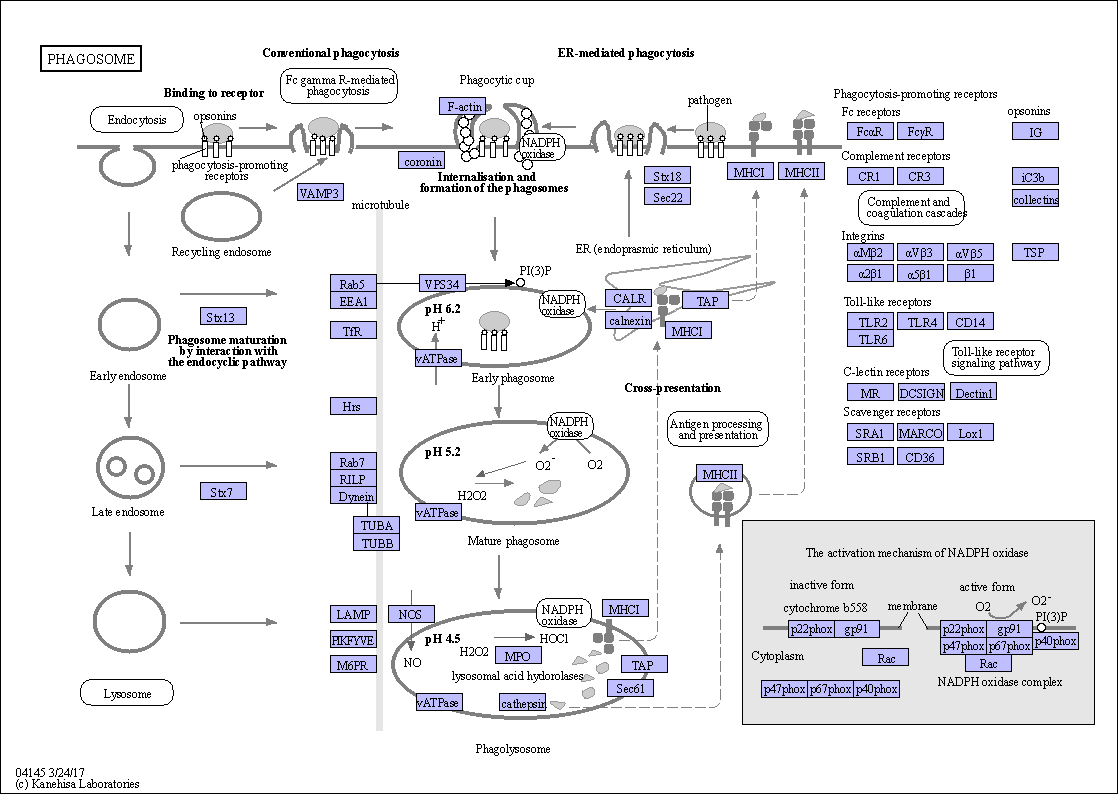
\includegraphics[width=\linewidth]{figs/ko04145.png}
            \caption{KEGG 2022 Phagosome\textsuperscript{*}}
            \tiny\textsuperscript{*} \url{https://www.genome.jp/kegg-bin/show_pathway?ko04145}
            \label{fig:kegg-2022-phagosome}
        \end{center}
\end{figure}
    \hypertarget{related-drugs}{%
\subsection{Related Drugs}\label{related-drugs}}

\hypertarget{quizartinib-and-crenolanib-flt3-inhibitors}{%
\subsubsection{Quizartinib and Crenolanib: FLT3
Inhibitors}\label{quizartinib-and-crenolanib-flt3-inhibitors}}

Mutations in the FLT3 gene occur in approximately one third of all
patients with newly diagnosed AML; 20\% to 25\% of these mutations are
ITD and 5\% to 10\% are point mutations of the tyrosine kinase domain.
Both types of mutations lead to constitutive activation of the FLT3
receptor tyrosine kinase, promoting cellular proliferation and survival
and inhibiting differentiation.\footnote{\href{https://aacrjournals.org/cancerdiscovery/article/10/4/506/2495/Advances-in-the-Treatment-of-Acute-Myeloid}{Advances
  in the Treatment of Acute Myeloid Leukemia: New Drugs and New
  Challenges}}

\hypertarget{venetoclax-bcl-2-inhibitors}{%
\subsubsection{Venetoclax: BCL-2
inhibitors}\label{venetoclax-bcl-2-inhibitors}}

Antiapoptotic proteins, including BCL2, BCL-XL, and MCL1, are frequently
overexpressed in AML and are associated with resistance to chemotherapy
(82). This observation led to the development of BH3 mimetics that
structurally mimic BH3-only proteins and are capable of binding to
antiapoptotic proteins, effectively inhibiting their functional activity
and inducing apoptosis.\footnote{\href{https://aacrjournals.org/cancerdiscovery/article/10/4/506/2495/Advances-in-the-Treatment-of-Acute-Myeloid}{Advances
  in the Treatment of Acute Myeloid Leukemia: New Drugs and New
  Challenges}}
\newpage
    \hypertarget{references}{%
\section{References}\label{references}}

\begin{itemize}
\tightlist
\item
  \href{https://maktabkhooneh.org/course/\%D8\%A8\%DB\%8C\%D9\%88\%D8\%A7\%D9\%86\%D9\%81\%D9\%88\%D8\%B1\%D9\%85\%D8\%A7\%D8\%AA\%DB\%8C\%DA\%A9-\%D9\%BE\%DB\%8C\%D8\%B4\%D8\%B1\%D9\%81\%D8\%AA\%D9\%87-mk375/\#seasons}{https://maktabkhooneh.org
  - Advanced Bioinformatics course}
\item
  \href{https://www.nature.com/scitable/definition/microarray-202/}{https://www.nature.com
  - microarray}
\item
  \href{https://www.digitalocean.com/community/tutorials/normalize-data-in-r}{https://www.digitalocean.com
  - How to Normalize data in R}
\item
  \href{https://www.v7labs.com/blog/data-preprocessing-guide}{https://www.v7labs.com
  - A Simple Guide to Data Preprocessing in Machine Learning}
\item
  \href{https://machinelearningmastery.com/dimensionality-reduction-for-machine-learning/}{https://machinelearningmastery.com
  - Introduction to Dimensionality Reduction for Machine Learning}
\item
  \href{https://towardsdatascience.com/11-dimensionality-reduction-techniques-you-should-know-in-2021-dcb9500d388b}{https://towardsdatascience.com
  - 11 Dimensionality reduction techniques you should know in 2021}
\item
  \href{http://www.sthda.com/english/articles/31-principal-component-methods-in-r-practical-guide/118-principal-component-analysis-in-r-prcomp-vs-princomp/}{http://www.sthda.com
  - Principal Component Analysis in R: prcomp vs princomp}
\item
  \href{http://www.sthda.com/english/articles/31-principal-component-methods-in-r-practical-guide/112-pca-principal-component-analysis-essentials/}{http://www.sthda.com
  - Principal Component Analysis Essentials}
\item
  \href{https://ajitjohnson.com/tsne-for-biologist-tutorial/}{https://ajitjohnson.com
  - Getting started with t-SNE for biologist (R)}
\item
  \href{https://towardsdatascience.com/t-sne-clearly-explained-d84c537f53a}{https://towardsdatascience.com
  - t-SNE clearly explained}
\item
  \href{http://www.sthda.com/english/articles/31-principal-component-methods-in-r-practical-guide/122-multidimensional-scaling-essentials-algorithms-and-r-code/}{http://www.sthda.com
  - Multidimensional Scaling Essentials: Algorithms and R Code}
\item
  \href{https://ucdavis-bioinformatics-training.github.io/2018-June-RNA-Seq-Workshop/thursday/DE.html}{https://ucdavis-bioinformatics-training.github.io/}
\item
  \href{https://www.nature.com/articles/s41467-020-14590-9}{FOXM1
  regulates leukemia stem cell quiescence and survival in MLL-rearranged
  AML}
\item
  \href{https://pubmed.ncbi.nlm.nih.gov/31943751/}{E2F4 functions as a
  tumour suppressor in acute myeloid leukaemia via inhibition of the
  MAPK signalling pathway by binding to EZH2}
\item
  \href{https://www.ncbi.nlm.nih.gov/pmc/articles/PMC8699747/}{The Role
  of T Cell Immunotherapy in Acute Myeloid Leukemia}
\item
  \href{https://www.frontiersin.org/articles/10.3389/fcell.2021.652972/full}{OGP46
  Induces Differentiation of Acute Myeloid Leukemia Cells via Different
  Optimal Signaling Pathways}
\item
  \href{https://aacrjournals.org/cancerdiscovery/article/10/4/506/2495/Advances-in-the-Treatment-of-Acute-Myeloid}{Advances
  in the Treatment of Acute Myeloid Leukemia: New Drugs and New
  Challenges}
\end{itemize}


    % Add a bibliography block to the postdoc
    
    
    
\end{document}
